\documentclass[12pt, a4paper,titlepage,openany]{article}
\usepackage[italian]{babel}
\usepackage[T1]{fontenc}
\usepackage[table]{xcolor}
\usepackage{float}
\restylefloat{table,figure}
\usepackage{graphicx}	
\usepackage[utf8]{inputenc}
\usepackage{amsmath}
\usepackage{fancyhdr}
\pagestyle{fancy}
\cfoot{\thepage}
\renewcommand{\footrulewidth}{0.25pt}
\usepackage{amssymb}
\usepackage{amsthm}
\usepackage{enumerate}
\usepackage{verbatim}
\title{Dispensa di Machine Learning}
\author{Federico Luzzi \\ Christian Uccheddu}
\date{}

\theoremstyle{plain}
\newtheorem{thm}{Teorema}[section]
\newtheorem{cor}[thm]{Corollario}
\newtheorem{lem}[thm]{Lemma}
\newtheorem{prop}[thm]{Proposizione}
\theoremstyle{definition}
\newtheorem{defn}{Definizione}[section]

\theoremstyle{remark}
\newtheorem{oss}{Osservazione}
\begin{document}
\maketitle

\tableofcontents
\clearpage
%\restylefloat{table,figure}
\pagestyle{fancy}
\cfoot{\thepage}
\renewcommand{\footrulewidth}{0.25pt}


\section{Dati}
Gli ambiti più importanti nei quali vengono applicate tecniche di machine learning nella vita reale sono diversi, in particolare si usano in:
finanza, sanità, agricoltura, e-commerce, social, chatbot, sensoristica (come i veicoli a guida autonoma).

Vista la grande mole di dati la necessità è capire come trattare i dati.

\textbf{L'obiettivo del Machine Learning è sviluppare metodologia per dare valore ai dati in funzione di una particolare domanda che ci stiamo facendo.}

Tipicamente le tecninche di machine learning si dividono nelle seguenti tre macro categorie:
\begin{itemize}
	\item Apprendimento supervisionato o predittivo: qualcuno ha gia catalogato ad esempio delle immagini o dei dati e noi prendendo questi modelli dovremmo essere in grado di predire.
	\item Apprendimento descrittivo: ci sono delle funzioni obiettivo che vanno ottimizzate. Non usiamo etichette della singola istanza ma in qualche modo sappiamo dove arrivare.
	\item Apprendimento rinforzato: E' quello più utile in questa epoca: funziona sui premi.
\end{itemize}

In questo corso ci concentreremo sui primi due tipi di apprendimento.

L' \textit{apprendimento supervisionato} si divide a sua volta nelle seguenti due categorie:
\begin{itemize}
	\item Classificazione: quando il problema consiste nel dividere in classi delle quantità discrete.
	\item Regressione: quando il problema consiste nel ricostruire una certa variabile date delle condizioni pregresse.
\end{itemize}

L' \textit{apprendimento non supervisionato} si divide a sua volta in:
\begin{itemize}
	\item Clustering: Quando il problema consistere nel ricostruire delle classi delle istanze che ci vengono consegnate, senza sapere nulla sulla storia pregressa.
	\item Associativa: Quando il problema consiste nel scoprire pattern che descrivono bene caratteristiche associate ad un certo fenomeno.
\end{itemize}

Per alcuni compiti la correlazione statistica va benissimo, in alcuni casi però essa è addirittura deleteria.  Se infatti provassi a vedere la correlazione tra il numero di omicidi in america e il numero di fondi investiti sulla ricerca scientifica vedrei che statisticamente sono strettamente correlate. Questo è un no-sense ed è il classico esempio di \textit{correlazione spuria.}

A confermare questa visione in cui il modello per una certa trattazione dati è fondamentale è il cosidetto paradosso di Simpson.

\textbf{Paradosso di Simpson:} Se uso solo i dati senza modello no c'è alcun modo di scoprire la verità.


\subsection{Data types}

Il primo passo fondamentale è sicuramente quello di prendere confidenza coi dati. E' fondamentale capire la natura intrinseca dei dati che abbiamo a disposizione, di solito essi sono organizzati in strutture che chiamiamo \textbf{dataset}. Per le analisi con le tecniche di Machine Learning esse non sono altro che tabelle fatte da righe e da colonne.

Le colonne del dataset sono chiamate \textbf{Attributi.}

Le righedel dataset sono chiamate \textbf{Istanze.}

Ogni attributo è caratterizzato dal fatto di avere un tipo, la sua conoscenza è fondamentale perché ci permette di sapere le proprietà che questo possiede.
In particolare gli attributi si dividono in due grandi gruppi:
\begin{itemize}
	\item Categorici:
	\begin{itemize}
		\item Nominali: ad esempio il colore degli occhi.
		\item Ordinali: ad esempio possono essere i giudizi.
	\end{itemize}
	\item Numerici:
	\begin{itemize}
		\item Intervallo: ammettono operazioni di somma e sottrazione. 
		\item Ratio: possiamo applicare tutte le operazioni logico/matematiche.
	\end{itemize}
\end{itemize}


\begin{figure}[H]
	\centering
	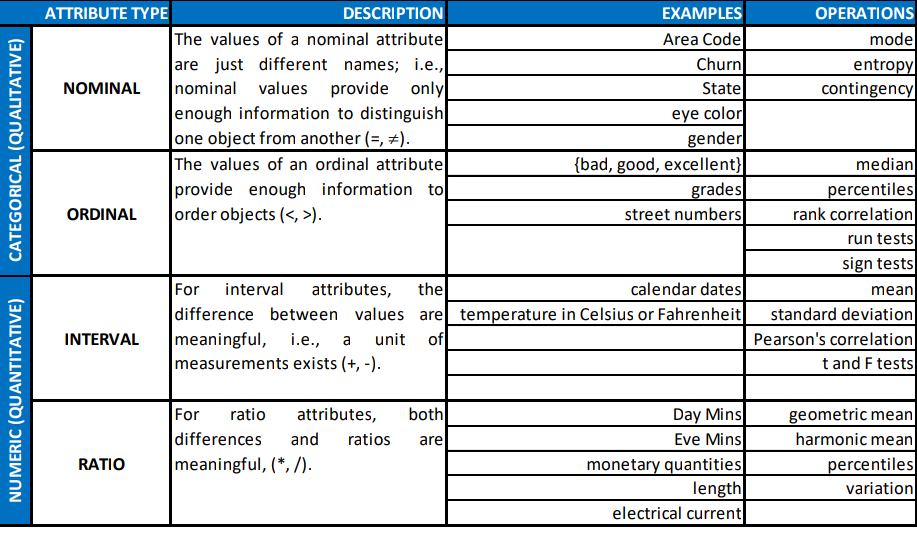
\includegraphics[height=0.5 \linewidth]{introduction/pict/attributi.png}
	\caption{Distinzione degli attributi con le relative proprietà}
\end{figure}
Dall'alto al basso il livello gerarchico sale e le proprietà aumentano.

C'è un'ulteriore divisione che può essere fatta ed è quella in:
Si possono anche dividere in attributi \textit{discreti} che possono essere:
\begin{itemize}
	\item Discreti (in cui la serie dei valori è finita o una infinità numerabile), che a loro volta si suddividono in:
	\begin{itemize}
		\item Categorici
		\item Numerici
		\item Binari: sono i più particolari da trattare, e hanno una serie di proprietà strane.
	\end{itemize}
	\item Continui, i cui valori sono numeri reali.
\end{itemize}

\subsection{Data exploration}

Dobbiamo però anche sapere come esplorare i dati in modo intelligente usando tutti i nostri strumenti a nostra disposizione. Diamo ora un elenco degli strumenti statistici più utili che ci permetton di avere un'analisi completa dei dati.

\subsubsection{Definizioni}
\begin{defn}
	Si definisce \textbf{quantile} $\alpha$ il valore $q_{\alpha}$ che divide la popolazione in due parti proporzionali rispettivamente ad $\alpha$ e a $(1 - \alpha)$ e caratterizzate da valori rispettivamente minori e maggiori di $q_{\alpha}$
\end{defn}

Un quantile molto importante è il quantile di ordine $\frac{1}{2}$ e si chiama \textbf{mediana} che è quello che ha esattamente minori di lui  metà dei dati.

\begin{defn}
	Si definisce \textbf{media} il seguente valore:
	\[mean = \frac{1}{n}\sum_{i=1}^{n}x_i\]
\end{defn}


La media non è un buon modo di visualizzare i dati perché dice poco riguardo alla loro distribuzione. Siccome la media è basata su singole osservazioni è fortemente soggetta a variazioni quando si hanno valori fortemente discostati dalla distribuzione dei dati.
Tali valori si chiamano \textit{outlier} e sono particolarmente interessanti da trattare.

Per ovviare a questo problema si è soliti usare  la \textbf{media trimmed} in cui si buttano via il valore più piccolo e il valore più grande. 
\begin{defn}
	Si definisce \textbf{media trimmed} il seguente valore:
	\[mean_{trimmed} = \frac{1}{n}\sum_{i=1}^{n}x_i  \qquad x_{i} = x - \max{x}- \min{x}\]
\end{defn}

Se si trova un grosso scostamento tra la media e la media trimmed probabilmente si ha la presenza di almeno un outlier.

\begin{defn}
	Si definisce \textbf{range} il seguente valore:
	\[ range = \max{x}- \min{x}\]
\end{defn}

Esso serve a quantificare la dispersione dei dati, ovviamente questo valore può essere fuorviante qualora i valori siano concentrati in una stretta banda di valori. Per ovviare a questo problema si usa la varianza.

\begin{defn}
	Si definisce \textbf{varianza} il seguente valore:
	\[ var =  \sigma^{2} =\frac{1}{n - 1 }\sum_{i = 1}^{n} (x_{i} - \bar{x})^{2}\]	
\end{defn}

E' preferibile però usare la deviazione standard in quanto per come è definita risulta essere della stessa unità di misura dei dati.
\begin{defn}
	Si definisce \textbf{deviazione standard} il seguente valore:
	\[ std = \sigma =  \sqrt{\sigma^{2}} \]
\end{defn}

Essendo queste due grandezze definite a partire dalla media esse soffrono dello stesso problema: sono fortemente condizionate dagli outlier, con lo stesso metodo precedente si definiscono quindi altre due grandezze in grado di ovviare a questo problema.

\begin{defn}
	Si definisce \textbf{deviazione media assoluta} il seguente valore:
	\[ AAD =  \frac{1}{n}\sum_{i=1}^{n}|x_i- mean|\]
\end{defn}

\begin{defn}
	Si definisce \textbf{deviazione mediana assoluta} il seguente valore:
	\[ MAD = mediana(x_{1}-mean, x_{2}-mean, ..., x_{n0}-mean )\]
\end{defn}

E' utile anche definire il range interquartile (IQR) sempre per ovviare alla presenza di outliar.

\begin{defn}
	Si definisce \textbf{deviazione mediana assoluta} il seguente valore:
	\[ IQR = q_{75\%} - q_{25\%}\]
\end{defn}

Ci sono anche diverse grandezze utili da definire nei casi in cui si ha a che fare con copppie di attributi, in tal caso:

\begin{defn}
	Si definisce \textbf{covarianza} il seguente valore:
\[cov(X,Y) = \frac{1}{m -1}\sum_{i = 1}^{m} (x_{i} - \bar{x})(y_{i} - \bar{y})\]
\end{defn}

Per come è costruita questa matrice è necessariamente quadrata, e il suo valore $ij ^{th}$ rappresenta la covarianza tra il valore $i^{th}$ dell'attributo x e il valore $j^{th}$ dell'attributo y.

Un'ulteriore misura dell'associazione tra le coppie di attributi quantitativi che non dipende dalla varianza di ciascun attributo è la seguente:

\begin{defn}
	Si definisce \textbf{correlazione di Pearson} il seguente valore:
	\[ corr(x,y) = \frac{cov(x,y)}{\sqrt{var(x)var(y)}}\]
\end{defn} 
Per come è definita si ha ovviamente che: $cov(x,y) \in [-1,1]$.

E' molto utile visualizzare i dati quando bisogna lavorarci, questo fondamentalmente per due motivi:
\begin{itemize}
	\item Ci permette di trovare pattern tra le variabili che valori puntuali non ci permetterebbero di trovare.
	\item Ci permette di visualizzare i risultati di una lavorazione fatta sui dati.
\end{itemize}

Di seguito proponiamo un rapido elenco dei grafici più utili e descriviamone le varie caratteristiche.

\subsubsection{Visualization}

Possono organizzare i dati in istogrammi caratterizzati dalla presenza di bin: essi indicano la larghezza in cui i dati sono organizzati. A seconda dell'ampiezza che uso posso ottenere due disegni molto diversi come mostrato in figura.


\begin{figure}[H]
	\centering
	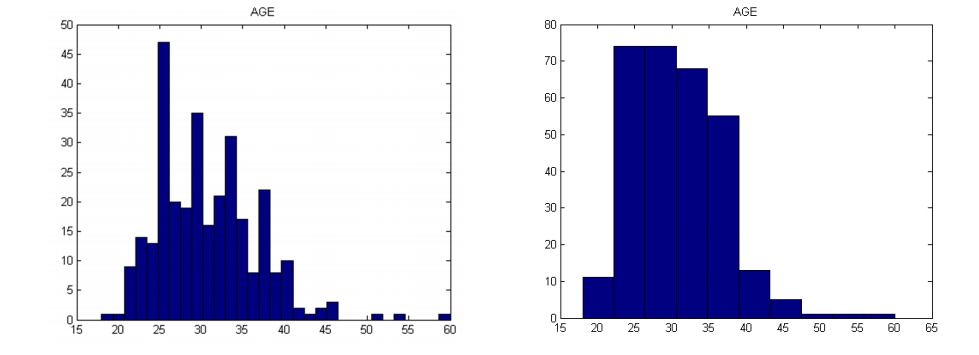
\includegraphics[height=0.35 \linewidth]{introduction/pict/istogramma_quant.png}
	\caption{Differenza tra due istogrammi fatti sulla stessa distribuzione di dati ma con numero di bin diversi.}
\end{figure}


Si possono allo stesso modo creare istogrammi per dati qualitativi. La differenza rispetto agli istogrammi sui dati quantitativi è quella per cui ogni bin corrisponde ad una categoria diversa.

\begin{figure}[H]
	\centering
	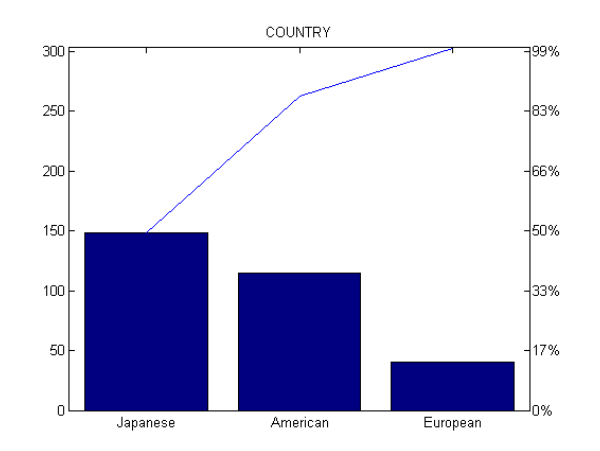
\includegraphics[height=0.3 \linewidth]{introduction/pict/istogramma_qual.png}
	\caption{Istogramma di dati qualitativi.}
\end{figure}

In questo caso la linea blu disegnata sopra è una linea cumulativa, ossia rappresenta dove si trova il livello sommando tutti i dati che man mano incontro, per come è costruita ovviamente dovrà finire sul valore $100\%$


Un altro modo di rappresentare i dati particolarmente utile è il \textbf{grafico Box and Whiskers} applicato solo ad attributi quantitativi. Rispetto agli istogrammi questo è decisamente più utilizzato perché permette di estrarre decisamente più informazioni. In particolare proponiamo un grafico in cui sono esplicitate le informazioni ottenibili:

\begin{figure}[H]
	\centering
	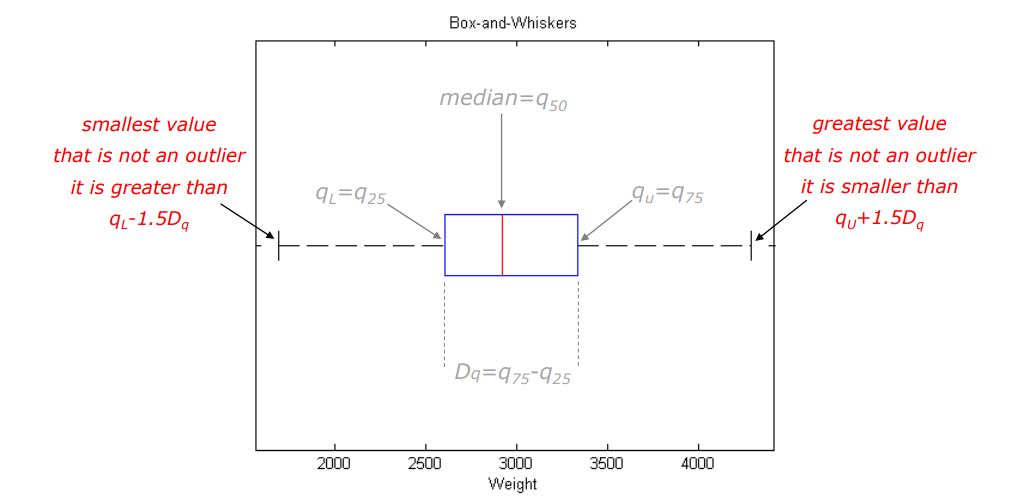
\includegraphics[height=0.4 \linewidth]{introduction/pict/box_plot.png}
	\caption{Informazioni ottenibili da un box plot.}
\end{figure}


\subsection{Missing replacement}

E' il problema che si occupa di studiare come sostituire i valori mancanti di certi attributi  in un dataset. Essendo un problema di così larga portata possiamo capire bene che una trattazione esaustiva riempirebbe le ore di un intero corso, tuttavia ne forniamo le basi per essere in grado di poter effettuare una analisi dati efficace. 

Le motivazioni principali del perché un database presenta delle mancanze sono le seguenti:
\begin{itemize}
	\item Tale valore non è stato possibile misurarlo.
	\item Non si conosce con esattezza tale valore.
	\item Si è verificato qualche errore durante la presa dati.
	\item Quel determinato attributo fino ad un certo punto dell'analisi non è mai stato considerati importante e quindi non è mai stato registrato.
\end{itemize}

Ci sono diversi metodi che ci permettono di riempire quel valore mancante, di seguito diamo una rapida trattazione dei più usati:

\begin{itemize}
	\item \textbf{Record removal:} è il metodo più drastico e consistere nell'eliminare tutta l'istanza che contiene quel valore. Non viene usato frequentemente perché si rischia di perdere valori che possono essere fondamentali per l'analisi dati.
	
	\item \textbf{Global constant:} consiste nel sostituire tutti i missing values con un valore costante chiamato \textit{place holder.} Tale metodo non è molto efficiente perché un valore costante non può essere rappresentativo di una distribuzione.
	
	\item \textbf{Manual inputation:} consiste nel sostituire manualmente i missing values tramite delle osservazioni. Lo svantaggio è che è tremendamente svantaggioso dal punto di vista computazionale.
	\item  \textbf{Moda replacement:} consiste nel rimpiazzare tutti i missing values con la moda di quel dato attributo, valgono le stesse considerazioni fatte per il metodo della global constant. Qualora gli attributi fossero continui si effettuerebbe la stessa cosa ma sostituendo la media.
	\item \textbf{Conditional mean replacement:} consiste nel rimpiazzare tutti i missing values con la media a condizione del fatto che sia presente un'ulteriore condizione posta su un secondo attributo. E' un po' più efficace degli altri elementi ma presenta anch'esso delle criticità.
	
	\item \textbf{Most probable:} consiste nel prendere un modello e sostituire quel valore.
\end{itemize}

E' ora chiaro che il confine tra l'esplorazione dati e la modellizzazione degli stessi è molto sottile.

\subsection{Data Preprocessing}

Tutti questi processi impattano fortemente tutta l'analisi che farò dopo.



ex}
\clearpage
%\restylefloat{table,figure}
\pagestyle{fancy}
\cfoot{\thepage}
\renewcommand{\footrulewidth}{0.25pt}


\section{Introduzione}
Gli ambiti più importanti nei quali vengono applicate tecniche di machine learning nella vita reale sono:
\begin{itemize}
	\item Finanza
	\item Sanità
	\item Agricoltura
	\item e-commerce
	\item Social
	\item Chatbot
	\item Sensoristica (come i veicoli a guida autonoma)
\end{itemize}

Vista la grande mole di dati la necessità è capire come trattare i dati.

\textbf{L'obiettivo del Machine Learning è sviluppare metodologia per dare valore ai dati in funzione di una particolare domanda che ci stiamo facendo.}

Tipicamente le tecninche di machine learning si dividono nelle seguenti tre macro categorie:
\begin{itemize}
	\item Apprendimento supervisionato o predittivo: qualcuno ha gia catalogato ad esempio delle immagini o dei dati e noi prendendo questi modelli dovremmo essere in grado di predire.
	\item Apprendimento descrittivo: ci sono delle funzioni obiettivo che vanno ottimizzate. Non usiamo etichette della singola istanza ma in qualche modo sappiamo dove arrivare.
	\item Apprendimento rinforzato: E' quello più utile in questa epoca: funziona sui premi.
\end{itemize}

In questo corso ci concentreremo sui primi due tipi di apprendimento.

L' \textit{apprendimento supervisionato} si divide a sua volta nelle seguenti due categorie:
\begin{itemize}
	\item Classificazione: quando il problema consiste nel dividere in classi delle quantità discrete.
	\item Regressione: quando il problema consiste nel ricostruire una certa variabile date delle condizioni pregresse.
\end{itemize}

L' \textit{apprendimento non supervisionato} si divide a sua volta in:
\begin{itemize}
	\item Clustering: Quando il problema consistere nel ricostruire delle classi delle istanze che ci vengono consegnate, senza sapere nulla sulla storia pregressa.
	\item Associativa: Quando il problema consiste nel scoprire pattern che descrivono bene caratteristiche associate ad un certo fenomeno.
\end{itemize}

Per alcuni compiti la correlazione statistica va benissimo, in alcuni casi però essa è addirittura deleteria.  Se infatti provassi a vedere la correlazione tra il numero di omicidi in america e il numero di fondi investiti sulla ricerca scientifica vedrei che statisticamente sono strettamente correlate. Questo è un no-sense ed è il classico esempio di \textit{correlazione spuria.}

A confermare questa visione in cui il modello per una certa trattazione dati è fondamentale è il cosidetto paradosso di Simpson.

\textbf{Paradosso di Simpson:} Se uso solo i dati senza modello no c'è alcun modo di scoprire la verità.


\subsection{Data Types}

Il primo passo fondamentale è sicuramente quello di prendere confidenza coi dati. E' fondamentale capire la natura dei dati che abbiamo a disposizione (\textbf{dataset}), c'è un fenomeno che si chiama \textbf{churn}, quando non siamo soddisfatti di un servizio ci affidiamo al competitor.

Ci possono essere valori missing in un dataset e possono mancare per diversi motivi.

Le colonne sono chiamate \textbf{Attributi.}

Le righe sono chiamate \textbf{Istanze.}

A volte ci sono anche attributi duplicati che possiamo tranquillamente buttare fuori.
Ogni attributo è caratterizzato dal fatto di avere un tipo. Conoscerlo è fondamentale per trattare i dati.
Gli attributi si dividono in due grandi gruppi:
\begin{itemize}
	\item Categorici:
	\begin{itemize}
		\item Nominali: ad esempio il colore degli occhi.
		\item Ordinali: ad esempio possono essere i giudizi.
	\end{itemize}
	\item Numerici:
	\begin{itemize}
		\item Intervallo: ammettono operazioni di somma e sottrazione. 
		\item Ratio: possiamo applicare tutte le operazioni logico/matematiche.
	\end{itemize}
\end{itemize}

Dall'alto al basso il livello gerarchico sale e le proprietà aumentano.

Si possono anche dividere in attributi \textit{discreti} che possono essere:
\begin{itemize}
	\item Categorici
	\item Numerici
	\item Binari: sono i più particolari da trattare, e hanno una serie di proprietà strane.
\end{itemize}
Oppure possono essere \textit{Continui.}

\subsection{Data exploration}

Dobbiamo però anche sapere come esplorare i dati. Per farlo facciamo cose molto elementari.
Per farlo si usano tutti gli strumenti a nostra disposizione.

Il concetto di \textbf{quantile} è trovare il numero di osservazione che ci indica quanti attributi sono più piccoli di un dato valore.
Un quantile molto importante è il quantile di ordine $\frac{1}{2}$ e si chiama \textbf{Mediana} che è quello che ha esattamente minori di lui la metà dei dati.

\[mean = \frac{1}{n}\sum_{i=1}^{n}x_i\]

La media non è un buon modo di visualizzare i dati perché dice poco ma quanto meno dice qualcosa. Siccome la media è basata su singole osservazioni si possono vedere le presenze di outliar, ossia di elementi troppo discordanti dalla media e che si presenta poche volte. Sono quindi elementi che è necessario trattare per vedere la provenienza.

Per prevenire questo si usa la \textbf{media trimmed} in cui si buttano via il valore più piccolo e il valore più grande. Se si trova un grosso scostamento probabilmente è presente un outlier.

Si puù definire anche il range anche se di solito si usa la varianza:
\[var = \frac{1}{n}\sum_{i = 1}^{n} (x_{i} - \bar{x})^{2}\]

Di solito si usa la deviazione standard che ha lo stesso ordine di grandezza dei dati:

\[ std = \sqrt{var} \]

Si usa anche il range interquartile (IQR) sempre per ovviare alla presenza di outliar.
Se ho a che fare con coppie di attributi allora è naturale parlare di \textbf{covarianza} ossia la varianza calcolata su due attributi diversi:

\[cov(X,Y) = \frac{1}{n}\sum_{i = 1}^{n} (x_{i} - \bar{x})(y_{i} - \bar{y})\]

Di solito si fanno scalature perché sennò le covarianze vengono troppo sbagliate. Per ovviare uso la \textbf{correlazione di Pearson} che può prendere valori $[-1,1]$
\[ corr(x,y) = \frac{cov(x,y)}{\sqrt{var(x)var(y)}}\]

Possono organizzare i dati in istogrammi in cui posso usare una ampiezza fissa o variabile (bin). A seconda dell'ampiezza che uso posso ottenere due disegni molto diversi.

Un altro modo di rappresentare i dati particolarmente utile è il \textbf{grafico Box and Whiskers} applicato solo ad attributi quantitativi.

\subsection{Missing replacement}

E' un problema enorme di per sè. Le operazioni più elementari sono le seguenti. In alcuni valori degli attributi un valore non è registrato. Ci possono esser tante ragioni: ad esempio un attributo non è sempre stato osservabile (penso all'ambito clinico), o ad esempio un attributo prima non veniva considerato rilevante.

Il primo nmetodo è il \textbf{Record removal} che è molto drastico come metodo perché comunque sia vengono eliminati dei valori che sarebbero potuti essere molto importanti.

Il secondo metodo è quello di \textbf{imputazione manuale}: è fatta da umani e tramite osservazioni ci si chiede se sia possibile inserirlo, è tremendamente difficile dal punto di vista computazionale.

Il terzo metodo è quello della \textbf{global constant}: ossia metto un numero là chiamato place holder con un valore costante, non troppo efficiente.

Il quarto metodo è quello di \textbf{rimpiazzarlo con la moda}, anche questo però è fortemente criticabile.
Se gli attributi sono continui si fa la stessa cosa ma con la media.

Il quinto metodo è \textbf{Conditional mean replacement} ossia bisogna rimpiazzare con la media solo se è presente un altro determinato attributo.

Il sesto metodo è quello del \textbf{most probable} ossia di prendere un modello e sostituire il valore.

E' molto difficile dare il confine tra l'esplorazione dei dati e la modellizzazione dei dati.

\subsection{Data Preprocessing}

Tutti questi processi impattano fortemente tutta l'analisi che farò dopo.




\section{Clustering}
\subsection{Introduzione(*)}

L'analisi di cluster è usata per risolvere moltissimi problemi pratici; in particolare, l'\textbf{analisi di cluster tratta due diversi scopi generali:}

\begin{itemize}
	\item \textbf{Comprensione}: Le classi, o gruppi di oggetti che condividono caratteristiche, giocano un ruolo importante nella comprensione del mondo. Questo succede in biologia, in informatica e in economia.
	\item \textbf{Utilità}: Capacità di riassumere determinate caratteristiche di un oggetto con le caratteristiche del cluster a cui appartiene. L'obiettivo è \textit{trovare i prototipi con le proprietà più rappresentative dei cluster}.
\end{itemize}

Può essere fornita una definizione un po' più completa di analisi di clustering come segue.
\begin{defn}
	La \textbf{cluster analysis} è la tecnica che raggruppa i dati basandosi sulle informazioni trovate nei dati che descrivono gli oggetti e le loro relazioni.
\end{defn}
Gli obiettivi sono semplici da ridefinire:
\begin{itemize}
	\item Gli oggetti all'interno di un gruppo devono essere simili gli uni con gli altri, allo stesso tempo diversi (o incorrelati) con gli oggetti di altri gruppi.
	\item La più grande \textit{similarità} entro un gruppo deve corrispondere ad una grande \textit{differenza} tra i gruppi. 
\end{itemize}

\textbf{Problema}: Come è possibile stabilire quando  e quanto degli oggetti sono simili? Non vi è un metodo per capirlo, tendenzialmente si utilizza una soluzione intermedia rispetto alle altre. 
\\La definizione di cluster è \textbf{intrinsecamente imprecisa},una migliore definizione dipende infatti dalla natura dei dati e dai risultati desiderati. 

\subsubsection{Tipi di clustering}

Formare un insieme di cluster è chiamato in gergo tecnico \textit{clustering.} Ci sono diversi tipi di analisi di clustering.

\begin{itemize}
	\item Partitional vs Hierarchical
	\item Exclusive vs  Overlapping vs Fuzzy
	\item Complete vs Partial.
\end{itemize}

Di seguito una rapida definizione di tutte:

\begin{defn}
	Un clustering si dice \textbf{partizionale} se vi è una divisione del dataset in insiemi non sovrapposti tali che un elemento appartiene ad un solo insieme.
\end{defn}

\begin{defn}
	Un clustering si dice \textbf{gerarchico} se ogni cluster può essere a sua volta suddiviso in sotto cluster, in questo caso il clustering è un insieme di cluster che sono organizzati come un albero.
\end{defn}

\begin{defn}
	Un clustering si dice \textbf{esclusivo} se ogni oggetto è assegnato ad un singolo cluster.
\end{defn}

\begin{defn}
	Un clustering si dice \textbf{sovrapponibile} se ogni oggetto può essere assegnato a più di un cluster.
\end{defn}

\begin{defn}
	Un clustering si dice \textbf{fuzzy} se ogni oggetto può essere assegnato a più di un cluster contemporaneamente con un valore che tiene conto del peso che ha l'oggetto rispetto all'appartenenza ad un singolo cluster, la somma dei pesi deve essere necessariamente 1.
\end{defn}
\begin{figure}[H]
	\centering
	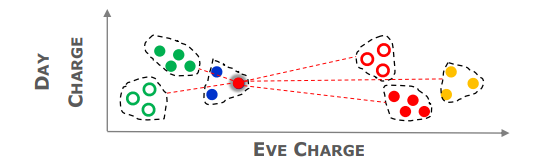
\includegraphics[height=0.3 \linewidth]{clustering/pict/fuzzy.png}
	\caption{Clustering con modello fuzzy}
\end{figure}
\begin{defn}
	Un clustering si dice \textbf{completo} se ogni oggetto è assegnato ad un cluster (non ci sono oggetti liberi).
\end{defn}

\begin{defn}
	Un clustering si dice \textbf{parziale} se esiste almeno un oggetto che non è assegnato a nessun cluster, si usa perché potrebbero esserci degli outlier ed inserirli all'interno di un cluster potrebbe peggiorare in modo significativo la rappresentazione di un cluster.
\end{defn}

\subsubsection{Differenti nozioni di cluster}
I cluster naturali sono cluster che si dicano esistano per davvero anche se è molto difficile che ciò accada. Per visualizzare le differenze tra i tipi diversi di dati si sfruttano dati come punti a due dimensioni. Le categorie in cui sono divisi gli algoritmi di clustering sono le seguenti:
\begin{itemize}
	\item \textbf{Well separated Cluster:} dato un cluster, ogni oggetto è più vicino ad ogni oggetto del cluster a cui appartiene piuttosto che a qualsiasi altro oggetto di ogni altro cluster. Un cluster così ben formato permette di avere separazioni molto nette, questo tipo di cosa succede però molto raramente in realtà.
	\item \textbf{Prototpe-based cluster} dato un cluster, ogni oggetto di quel cluster è più vicino al prototipo che definisce il cluster rispetto ad ogni prototipo di un altro cluster. Il prototipo \`e solitamente il \textit{centroide} del cluster. Il \textit{prototipo} di un cluster corrisponde all'individuo meglio rappresentato dal cluster (può essere anche fittizio). Cluster fatti in questo modo tendon ad essere globulari.
	\item \textbf{Density-based cluster} un cluster è una regione densa di oggetti che sono circostritti da una regione di bassa densità. Questi sono usati quando i cluster sono irregolari o intermittenti oppure quando c'è una grande presenza di rumore o di outlier.
	\item \textbf{Graph-based cluster} se i dati sono rappresentati da grafi, i nodi rappresentano  oggetti e i collegamenti connettono gli oggettti. Allora ogni cluster è una componente connessa. La connessione può anche essere pesata e scelta in base ad una certa soglia. 
	Questi cluster sono molto utilizzati in quanto c'è un sacco di ricerca già fatta.
\end{itemize}

\subsubsection{Componenti di un'analisi di clustering}

La prima fase di un'analisi di clustering consiste nella \textit{feature selection} che assicura la trattenuta degli attributi del dataset degni di significato. Successivamente avviene la fase di  \textit{feature extraction} che serve a produrre feature che potrebbero andare meglio per scoprire la struttura dei dati, questa pratica potrebbe tuttavia generare features di difficile comprensione.
Bisognerebbe usare come feature ideali quelle che permettono di distinguere i pattern degli elementi che appartengono ai diversi cluster, immuni al rumore e facili da interpretare.

Il secondo passo è quello di \textit{determinare la misura di prossimità e costruire la funzione di merito.} Una volta che abbiamo determinato una misura di prossimità il problema di clustering si traduce in un problema di ottimizzazione di una specifica funzione.

Bisogna ricordare sempre che diversi algoritmi di clustering portano ad avere conclusioni anche totalmente diverse, questo è il motivo per cui in principio non bisogna prediligere alcun algoritmo ma confrontare i risultati ottenuti e trarne conclusioni.


\subsection{Proximity(*)}

La proximity è uno strumento fondamentale per valutare il funzionamento di un algoritmo di clustering. Questa influenza, quindi, in modo pesante la soluzione di un problema di clustering. Bisogna fare una scelta della misura con cui si approssima la similarità degli elementi appartenenti allo stesso cluster.

\subsubsection{Introduzione}
\textit{La analisi dei cluster affonda le sue radici nel concetto di cosa sia simile e cosa sia dissimile,} l'analisi di questo concetto  in termini formali diventa abbastanza difficile. Questo avviene perché la similitudine dipende fortemente dal contesto analizzato.

\textit{In generale la similarità è nulla se i due oggetti sono totalmente differenti sotto la caratteristica che stiamo valutando ed è uguale a 1 se sono completamente uguali, è comune però trovare misure di similitudine che hanno come valori:  $[0,\inf]$.} Useremo il termine \textbf{proximity} per indicare sia la similarità che la dissimilarità. 

\begin{figure}[H]
	\centering
	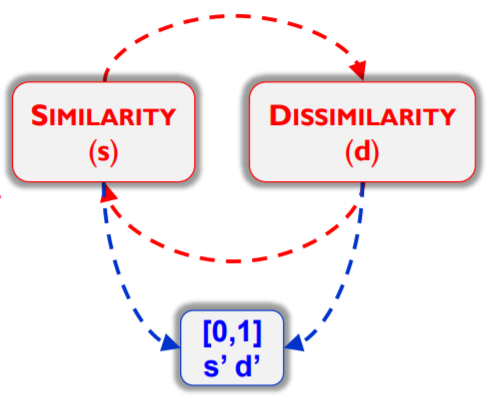
\includegraphics[height=0.45 \linewidth]{clustering/pict/simil_diss.png}
	\caption{Relazione tra similarità e dissimilarità}
\end{figure}

Non c'è ortogonalità tra la scelta della misura e l'esito che otterrò; nasce, per questo motivo, l'esigenza di poter passare da una misura all'altra, in particolare, per trasformare una misura di similarità dall'intervallo $[0,\inf]$ all'intervallo $[0,1]$ si opera la seguente trasformazione:

\[s' = \frac{s - \min{s}}{\max{s} - \min{s}} \qquad d' = \frac{d - \min{d}}{\max{d} - \min{d}} \] 

Ci sono diversi problemi che nascono quando viene cambiato l'intervallo in cui si trova il valore. Per farlo bisogna usare una trasformazione \textit{non-lineare}. Possono essere usati, però,  funzioni del genere:

\[ d' = \frac{d}{1+d}\]

Con questa trasformazione grandi valori della dissimilarità $d$ vengono compressi in valori vicini a 1. Il fatto di distorcere o meno le distanze dipende dal compito che bisogna svolgere.
Ci sono diversi problematiche che nascono quando si trasforma una similarità in dissimilarità e viceversa. Per farlo bisogna usare una trasformazione \textit{non-lineare}. Si può usare, però, una cosa del genere:

\[ se \quad s,d = [0, 1]  \quad allora  \quad s =  1-d\]

\textit{In generale si può usare qualsiasi funzione monotona decrescente per trasformare la similarità in dissimilarità.}

\begin{defn}
	Si definisce \textbf{prossimità} tra due record come la funzione di prossimità tra i corrispondenti attributi dei due record.	
\end{defn}

Si consideri in prima analisi la misura di prossimità tra due record aventi un solo attributo ed estendiamo successivamente questa analisi a record con più di un attributo.
\begin{figure}[H]
	\centering
	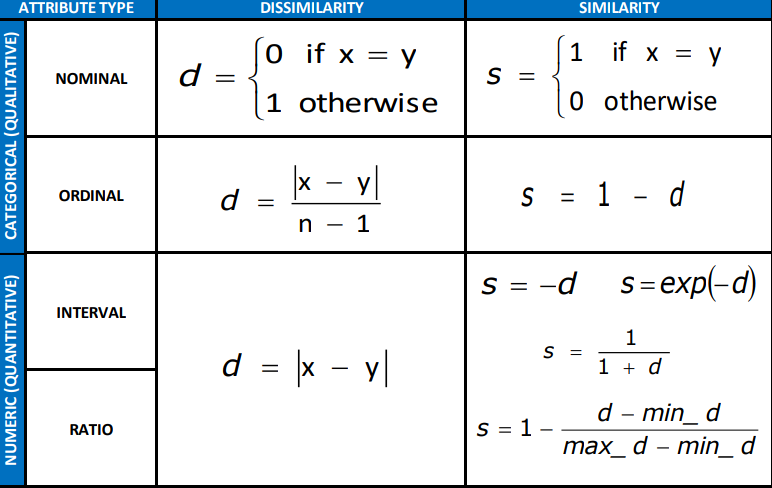
\includegraphics[height=0.3 \linewidth]{clustering/pict/proximity_one.png}
	\caption{Tabella per misurare la prossimità di record con un solo attributo in funzione del tipo di attributo}
\end{figure}

Si considerino due record riferiti al medesimo attributo nominale qualitativo, tutto ciò che si può dire è se i due record abbiano lo stesso valore o meno.
Per quanto riguarda gli attributi binari la dissimilarità esclude la similarità con valori 0 e 1. 

Se ho attributi categorici ordinali assegno un valore intero agli stessi in base alla scala utilizzata e calcolo la dissimilarità come rapporto tra la differenza dei due record e la scala totale di valori di utilizzo. Naturalmente va notato che sto utilizzando una scala lineare, questa è ovviamente un'assunzione molto forte che però bisogna tenere in conto in quanto qualsiasi scala di valori scelta è fatta basandosi su assunzioni.

Come si nota dalla tabella è molto più facile definire la prossimità tra due attributi numerici, essa è infatti definita come \textit{la differenza in modulo tra i due valori.}
\subsubsection{Misure della distanza}

Quando si hanno degli attributi numerici possono essere definite altre misure di distanza nel seguente modo:
\begin{figure}[H]
	\centering
	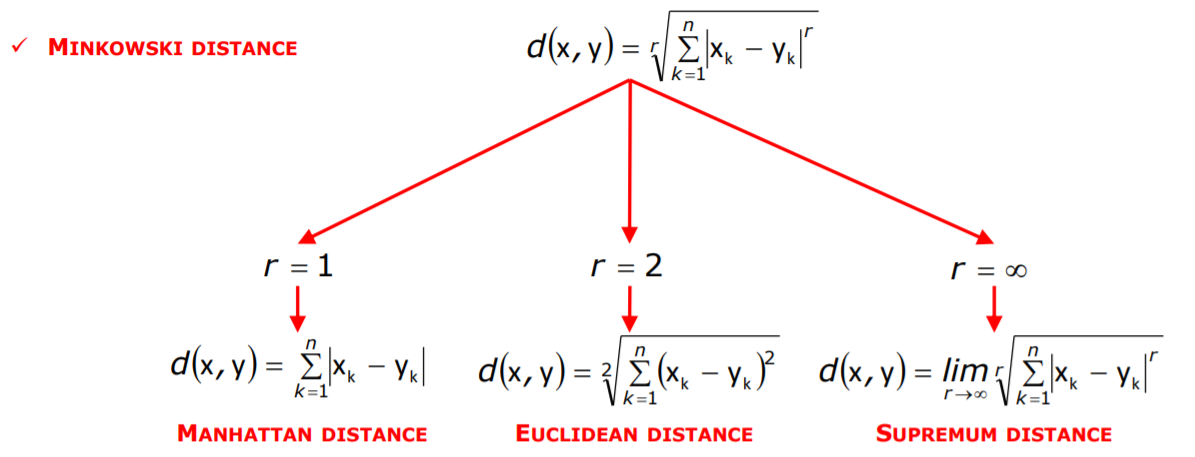
\includegraphics[height=0.3 \linewidth]{clustering/pict/distanze_minkowski.png}
	\caption{Misure di distanza a partire dalla distanza di Minkowski}
\end{figure}
Le proprietà che una funzione deve soddisfare per essere definita distanza sono le seguenti:
\begin{itemize}
	\item Non negatività: $d(x,y) \geq 0 \quad \forall x,y \quad d(x,y) = 0 \quad if \quad x = y$
	\item Simmetria $d(x,y) = d(y,x) \quad \forall x,y$
	\item Disuguaglianza triangolare $d(x,z) \leq d(x,y) + d(y,z) \quad \forall x,y,z$
\end{itemize}

 \textit{La similarità generalmente non rispetta la disuguaglianza triangolare ma solitamente verifica le proprietà di simmetria e non negatività.}

Di seguito qualche esempio di misura di prossimità:
\begin{defn}
	 Si definisce \textbf{Simple matching coefficient} la seguente espressione: \[ SMC(x,y) = \frac{\#maching\_attributes}{\#attributes} =  \frac{f_{11}+ f_{00}}{f_{11}+ f_{00} + f_{01}+ f_{10}} \]
\end{defn}
Questa è una misura che ha senso per attributi \textit{simmetrici binari}, ossia per attributi che possono assumere solo i valori 0 o 1 in circa egual quantità.
 Questa misura è invece scomoda se non si può affermare se gli 0 siano veramente degli 0, per il valore 1 invece è chiaro. In questo caso si utilizza un'altra misura che è derivata da questa misura, ossia si usa l'assunzione per cui l'osservazione di un evento (identificata con 1), abbia peso maggiore della non osservazione di un evento (rappresentata con 0). Si definisce quindi il coefficiente di Jaccard nel seguente modo:

\begin{defn}
	Si definisce \textbf{Jaccard Coefficient} la seguente espressione:    \[ J(x,y) = \frac{\#maching\_attributes}{\#attributes\_except00} = \frac{f_{11}}{f_{11}+ f_{01}+ f_{10}}\]
\end{defn}


Questa è ovviamente una misura distorta rispetto agli 1 (infatti è un tipo di misura che va bene con attributi \textit{asimmetrici}) che permette, però, di focalizzare la attenzione sulla presenza di questi ultimi. Di seguito la definizione di un nuovo indice:

\begin{defn}
	Si definisce \textbf{Extended Jaccard Coefficient} la seguente espressione: \[ EJ(x,y) = \frac{x \cdot y}{||x||^2 + ||y||^2 - x \cdot y}\]
\end{defn}

 Questa misura è distorta per trattare dati sparsi, quindi tanti elementi in cui sono presenti 0 e solo poche diverse da 0, questo si usa ad esempio nell'analisi del linguaggio naturale. Si pensi ad esempio ai tweet, una parola presente in una frase ha una rilevanza maggiore rispetto ad una parola non presente nella stessa frase.

\subsubsection{Altre misure di prossimità}
Di seguito vengono proposte ulteriori misure di prossimità.
\begin{defn}
	Si definisce \textbf{cosine similarity.} la seguente espressione:   \[ cos(x,y) = \frac{x \cdot y }{||x|| \cdot ||y||  } \]
\end{defn}

 Questa misura viene usata quando tutti gli attributi sono di natura numerica, e si ignorano i match di natura 00. Il vantaggio di questa misura rispetto a quella di Jaccard è che in grado di trattare anche attributi non binari. E' molto utile quindi per comparare record sparsi ed è molto usata in \textit{Information Retrieval} dove i documenti (rappresentati come conteggi di vettori) devono essere comparati.

\begin{defn}
	Si definisce \textbf{Correlazione} la seguente espressione:    \[ corr(x,y) = \frac{cov(x,y)}{std(x)std(y)}\]
\end{defn}
Questa è la stessa correlazione di Pearson ma non legata alle variabili aleatorie.

Di seguito diverse \textbf{problematiche} legate alle misure di prossimità:
\begin{itemize}
	\item Come si trattano attibuti su scale di ampiezza diverse e/o correlati?
	
	Per risolvere il primo problema viene fatta la seguente cosa: si normalizzano i valori, se ciò non venisse fatto le distanze Euclidee tra i due valori risulterebbero totalmente distorte a favore del valore maggiore. 
	
	Quando gli attributi sono fortemente correlati invece il trucco sta nel fatto che la misura di similarità è molto simile al grado di correlazione tra questi attributi, in tal caso si utilizza la distanza di Mahalanobis:
	
	\[Mahal(x,y) = (x- y)\Sigma^{-1}(x- y)^{T}\]
	
	Ovviamente questa è una distanza che va usata solo se tutti gli attributi sono numerici.
	\item Come si calcola la prossimità tra record composti da attributi di tipo diverso?
	
	 Per risolvere questo problema si valutano tutte le misure di prossimità enunciate in precedenza stando coerenti col tipo di attributo trattato.  
	Dopo averlo fatto si usa una variabile indicatrice $\delta_{k}$ per ogni attributo k come segue:
	
	$\delta_{k}$ vale:
	\begin{itemize}
		\item 0  se il k-esimo attributo è asimmetrico ed entrambi i valori hanno  valore 0,  o almeno uno dei record presenta un missing value
		\item 1 altrimenti.
	\end{itemize} 


	Una volta definite queste allora la similarità si calcola come:
	\[similarity(x,y) = \frac{\sum_{k=1}^{n}\delta_{k}s_{k}(x,y)}{\sum_{k=1}^{n}\delta_{k}}\]
	\item Come si tratta la prossimità quando gli attributi hanno diversa rilevanza, ossia quando gli attributi contribuiscono secondo pesi diversi all'analisi? 
	
	Per risolvere quest'ultimo problema si procede esattamente nel modo precedente assegnando però dei pesi, le formule risolutive diventano quindi:
	\[similarity(x,y) = \frac{\sum_{k=1}^{n}w_{k}\delta_{k}s_{k}(x,y)}{\sum_{k=1}^{n}\delta_{k}}\]
\end{itemize}

Come è facilmente intuibile risulta molto complesso sostenere tutta questa specificità. Per farlo si cerca di ricondursi alla seguente scelta:
\begin{itemize}
	\item Dati densi e continui: distanze metriche  come quella euclidea sono buone rappresentazioni.
	\item Dati sparsi, binari asimmetrici: misure della distanza che ignorano i match 00 come cosine, Jaccard e Extended Jaccard.
\end{itemize}

\subsection{Clustering Algorithms}
Di seguito la trattazione degli algoritmi di Clustering veri e propri:
\subsubsection{Prototype Based}

L'approccio ai  \textit{Prototype-Based Clustering} si basa sull'assunzione che ogni cluster possa essere ben rappresentato da un unico punto chiamato \textbf{prototipo.} Ogni oggetto è quindi collocato nel cluster del prototipo a cui è più vicino.

\begin{figure}[H]
	\centering
	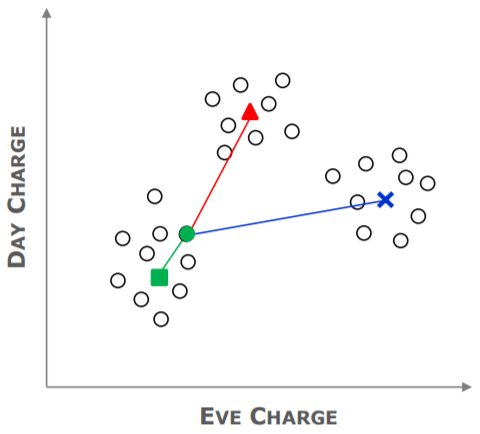
\includegraphics[height=0.4 \linewidth]{clustering/pict/prototype_cluster.png}
	\caption{Esempio di prototype-based clustering}
\end{figure}
Esistono diversi tipi di algoritmi basati sul prototipo a seconda delle seguenti caratteristiche:

\begin{itemize}
	\item Ogni oggetto deve appartenere ad un singolo cluster.
	\item Ogni record è nella condizione di appartenere a più di un cluster contemporaneamente.
	\item Il concetto di cluster è modellizzato con una distribuzione di tipo probabilistico.
	\item I cluster sono costretti ad avere relazioni fissate.
\end{itemize}

\paragraph{K-medie}

Di seguito viene proposta la descrizione di uno dei primi algoritmi basati sul prototipo. In questo caso il prototipo prende il nome di \textit{centroide;} questo valore solitamente è identificato dal vettore media dei valori degli attributi delle osservazioni di quel determinato cluster. Non c'è vincolo a ragionare in due dimensioni, il cluster generalmente è applicato ad oggetti in uno spazio continuo n-dimensionale.

Di seguito una descrizione schematica dell'algoritmo:
\begin{itemize}
	\item Scegliere per $k = 0$ quali sono i centroidi facendo in modo che non si "pestino i piedi".
	\item \textbf{Ripetere:}
	\begin{itemize}
		\item Formare k cluster in modo da assegnare ad ogni record il suo centroide più vicino. E' ovviamente un meccanismo esclusivo.
		\item Calcolare il nuovo centroide per ogni cluster .
		\item \textbf{Finché} il centroide non cambia più.		 
	\end{itemize}
	
	
\end{itemize}

Come si nota facilmente, bisogna esplicitare il numero di cluster prima dell'esecuzione dell'algoritmo; valori di partenza differenti possono fornire risultati molto diversi. La scelta del numero di cluster è dunque un ambito da tenere fortemente in considerazione.

L'algoritmo delle K-medie non è vincolato ad utilizzare la distanza Euclidea ma possono essere utilizzate le diverse misure di prossimità utilizzate in precedenza. In particolare:

\begin{itemize}
	\item \textbf{Manhattan:} in questo caso si utilizzano le mediane come centroidi, l'obiettivo è quindi \textit{minimizzare la somma delle $L_{i}$ distanze dei record rispetto al centroide del cluster a cui appartiene.}
	\item \textbf{Squared Euclidea:} in questo caso si utilizzano le medie come centroidi, l'obiettivo è quindi \textit{minimizzare la somma delle $L_{i}$ distanze dei record rispetto al centroide del cluster a cui appartiene.}
	\item \textbf{Cosine:} in questo caso vengono utilizzate le medie come centroidi, l'obiettivo è quindi \textit{massimizzare la somma delle cosine similarity dei record rispetto al centroide del cluster a cui appartiene.}
\end{itemize}


Di seguito tutta una serie di \textbf{problematiche} relative all'utilizzo dell'algoritmo delle K-medie come algoritmo di clustering.
\begin{itemize}
	\item\textit{Scelta dei centroidi iniziali:} è una fase fondamentale e influenza in modo pesante le performance dell'algoritmo in generale. Se si opta infatti per una scelta random dei centroidi iniziali si possono avere cluster molto diversi. Vi sono diverse alternative per ovviare a questo problema quali il clustering gerarchico.
	\item \textit{Complessità spaziale e temporale:} questi sono due punti a favore del K-medie. In particolare occupa pochissimo spazio in quanto vengono salvate solo le posizioni dei centroidi; inoltre, si tratta di un algoritmo abbastanza rapido in quanto è lineare rispetto al numero di istanze considerate. 
	\item \textit{Cluster vuoti:} bisogna tenere in considerazione che può capitare che un cluster sia vuoto per scelta sbagliata di centroidi iniziali (magari randomica).
	\item \textit{Presenza di outlier:} Questi elementi creano grossi problemi nel calcolo della media delle osservazioni di un cluster. Risulta efficiente però nella ricerca di outlier in quanto verranno identificati come cluster di singleton. Risulta spesso utile rimuoverli.
\end{itemize}

Di seguito una serie di \textbf{limiti} riferiti alla ricerca dei cluster con l'algoritmo delle k-medie:
\begin{itemize}
	\item Diffiicoltà  a ricercare cluster di non forma sferica. 
\begin{figure}[H]
	\begin{minipage}[b]{0.5\textwidth}
		\centering
		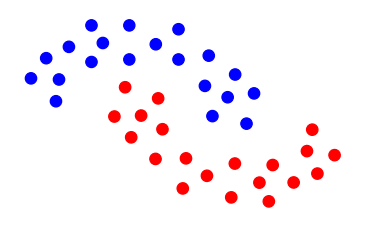
\includegraphics[width=0.7\textwidth]{clustering/pict/non_sferica_1.png}
		\caption{Cluster non sferico.}
	\end{minipage}
	\hfill
	\begin{minipage}[b]{0.5\textwidth}
		\centering
		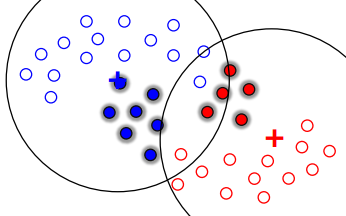
\includegraphics[width=0.7\textwidth]{clustering/pict/non_sferica_2.png}
		\caption{Cluster sferico.}
	\end{minipage}
\end{figure}
	
	\item Difficoltà a trovare cluster con dimensioni diverse: questo problema nasce dal fatto che la distanza è fissata.
	\begin{figure}[H]
		\begin{minipage}[b]{0.5\textwidth}
			\centering
			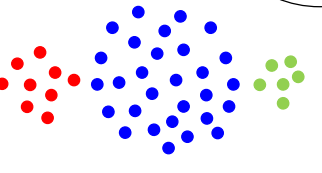
\includegraphics[width=0.7\textwidth]{clustering/pict/distanza_fissata_1.png}
			\caption{Distanza non fissata.}
		\end{minipage}
		\hfill
		\begin{minipage}[b]{0.5\textwidth}
			\centering
			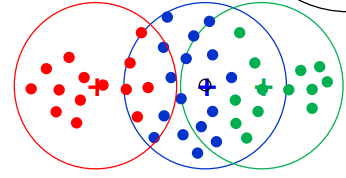
\includegraphics[width=0.7\textwidth]{clustering/pict/distanza_fissata_2.png}
			\caption{Distanza fissata.}
		\end{minipage}
	\end{figure}
	\item Difficoltà a indentificare cluster di diversa densità: questo prblema nasce dal fatto che i cluster possono avere dimensioni nettamente diverse.
	\begin{figure}[H]
		\begin{minipage}[b]{0.50\textwidth}
			\centering
			
\includegraphics[width=0.7\textwidth]{clustering/pict/densita_1.png}
			\caption{Densità differenti.}
		\end{minipage}
		\hfill
		\begin{minipage}[b]{0.50\textwidth}
			\centering
			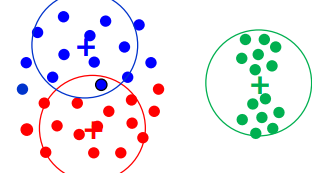
\includegraphics[width=0.7\textwidth]{clustering/pict/densita_2.png}
			\caption{Densità simili.}
		\end{minipage}
	\end{figure}
\end{itemize}
Come si può notare queste tre problematiche  portano a considerare cluster notevolmente differenti. Esiste un modo di risolvere parzialmente queste problematiche: \textit{accettare un clustering che rompe i cluster naturali in un numero variabile di sottocluster.}

Di seguito un rapido elenco che riassume \textbf{punti di forza e debolezze} dell'algoritmo delle k-medie:
\begin{itemize}
	\item Semplice e si applica a tanti tipi di dati.
	\item Abbastanza efficiente anche se vengono ripetute molte cose.
	\item Vi sono varianti più efficienti e meno problmatiche come ad esempio l'algoritmo \textit{bisecting k-means.}
	\item Non adatto a tutti i tipi di dati e non può gstire cluster non sferici, con size e densità diverse.
	\item Problemi con outliers.
	\item Strettamente legato al concetto di centroide. Vi sono delle varianti che utilizzano il \textit{medoide} e che sono più efficienti.
	
	
\end{itemize}

\paragraph{Fuzzy C-means}
Se gli elementi sono distribuiti in gruppi ben separati il clustering è semplice e vengono messi in cluster disgiunti. In molti casi succede però che i record non possano essere partizionati in cluster ben separati, nasce quindi un'incertezza arbitraria nell'assegnare gli oggetti ad un particolare cluster. Questa problematica si riflette infatti sulla scelta dell'assegnazione degli elementi di frontiera al rispettivo cluster.

\begin{figure}[H]
	\centering
	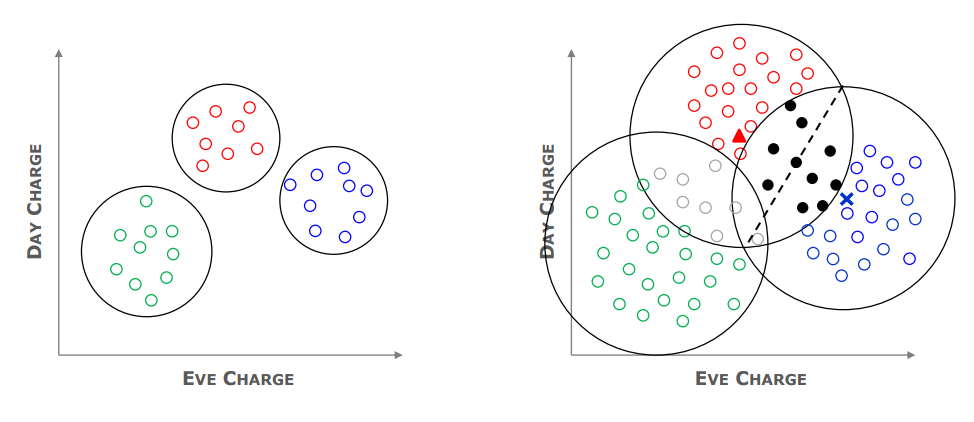
\includegraphics[height=0.4 \linewidth]{clustering/pict/frontiera.png}
	\caption{Differenza tra cluster ben separati e non ben separati.}
\end{figure}
Per ovviare al problema ogni osservazione viene considerata come appartenente ad ogni cluster ma con un peso diverso che indica il grado con cui un oggetto appartiene ad un ogni cluster. In particolare $w_{ij}$ è il \textit{peso} con cui l'$i$-esimo oggetto appartiee al $j$-esimo cluster.

Si assuma di avere un dataset di $m$ oggetti/record, dove ogni oggetto è associato ad un numero dato di attributi continui.

\begin{defn}
	Si definisce \textbf{Fuzzy pseudo-partition} l'assegnazione dei valori dei pesi $w_{ij}$ con i seguenti vincoli:
	\[\sum_{j = 1}^{K}w_{ij} = 1 \quad i=1,2,...,m\]
	\[0 < \sum_{i = 1}^{K}w_{ij} <  m \quad j=1,2,...,K\]
\end{defn} 

Ovviamente per come sono definiti i cluster \textit{non vengono ammessi cluster a dimensione nulla.} Il Fuzzy C-means \textit{produce dunque un clustering che risalta l'indicazione del grado per cui un oggetto appartiene ad ogni cluster.} Per come è definito ha gli stessi punti di forza e debolezze dell'algoritmo delle k-medie sebbene sia computazionalmente più pesante.

\paragraph{Modelli a mistura}
I modelli a mistura considerano i dati come insiemi di osservazioni da una mistura di diverse distribuzioni di probabilità.  In sostanza si possono considerare le misture come distribuite secondo delle normali con uguale varianza ma medie diverse (curve di livello). 

\begin{figure}[H]
	\centering
	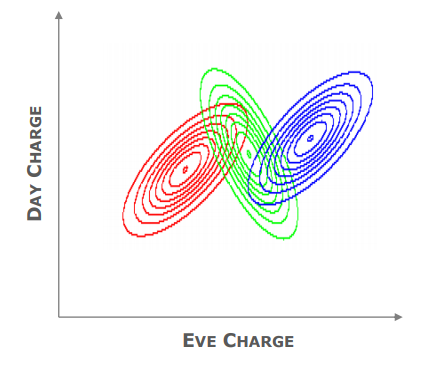
\includegraphics[height=0.3 \linewidth]{clustering/pict/mixture.png}
	\caption{Curve di livello nei modelli a mistura.}
\end{figure}

Si supponga di avere uno spazio a 3 componenti, il processo di generazione delle curve di livello è il seguente:
\begin{enumerate}
	\item Selezione di  una delle 3 componenti.
	\item Estrazione di un campione dalla componente selezionata.
	\item Ripetere 1 e 2 m volte per ottenere il dataset.
\end{enumerate} 

Vengono inoltre le seguenti grandezze:

\begin{itemize}
	\item $p(\bar{x}|\Theta) = \sum_{j=1}^{K} w_j p(\bar{x}|\theta_j)$: probabilità associata all'oggetto x.
	\item $w_j$: probabilità della j-esima componente.
	\item $p(\bar{x}|\theta_j)$: probabilità di estrarre x dalla j-esima componente.
	\item $\theta_j$: parametri associati a j.
\end{itemize}
Il processo consiste nel partire dai dati e ridurli nelle misture significative.
Esiste un classe di algoritmi utilizzata per la risoluzione di questo problema che è l'\textbf{Expectation Maximization}. Si tratta di algoritmi che sono diversi in base alla loro applicazione. 

\begin{figure}[H]
	\centering
	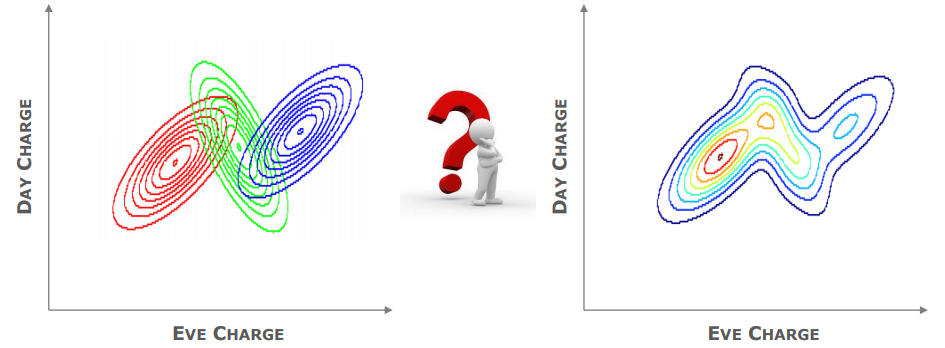
\includegraphics[height=0.3 \linewidth]{clustering/pict/expectation_maximization.png}
	\caption{Risultato auspicabile.}
\end{figure}
Questa classe di algoritmi presenta però diversi \textbf{svantaggi:}

\begin{itemize}
	\item L'apprendimento risulta essere molto lento.
	\item Non è pratico per i modelli con un gran numero di componenti.
	\item Non funziona bene quando i cluster contengono  poche osservazioni.
	\item Non funziona bene quando gli oggetti sono co-lineari.
\end{itemize}

Questi algoritmi presentano però anche una serie di \textbf{vantaggi} non indifferenti rispetto a quelli delle k-medie:
\begin{itemize}
	\item Sono più generali rispetto alle k-medie e alle fuzzy perché usano distribuzioni di vario tipo, possono trovare cluster di diversa grandezza e di forma ellittica.
	\item Disciplina il metodo di eliminazione delle complessità associate ad alcuni tipi di dati.
\end{itemize}

\paragraph{Mappe di Kohonen o SOMs}
E' una struttura feedforward per algoritmi di clustering; in particolare, viene imposta un'organizzazione topografica dei \textit{neuroni} (centroidi). Durante il processo di training la SOM usa ogni oggetto per aggiornare il centroide più vicino e i centroidi che sono più vicini nell'ordinamento topografico.
La differenza principale tra gli algoritmi precedenti è che i centroidi in questo caso \textit{hanno una predeterminata relazione di ordinamento topografico.}

In particolare, si ha che i centroidi che sono più vicini l'uno all'altro nella griglia sono più strettamente correlati rispetto ai centroidi che sono lontani.
\begin{figure}[H]
	\centering
	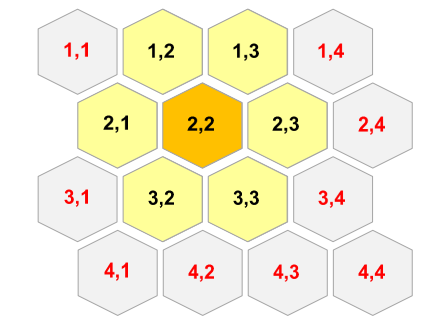
\includegraphics[height=0.3 \linewidth]{clustering/pict/som.png}
	\caption{Girglia di una SOM.}
\end{figure}

A causa di questo vincolo i centroidi di una griglia bidimensionale possono essere visti come giacenti su una \textit{superficie bidimensionale che prova ad adattare i dati multidimensionali il meglio possibile.}

Si riassumono di seguito i passaggi con cui una SOM crea i cluster:
\begin{enumerate}
	\item \textit{Inizializzazione:} vengono selezionati i centroidi associati a ciascun neurone
	\item \textit{Competizione:} i neuroni competono tra loro per ottenere l'istanza. Ogni neurone fa un'offerta diversa per vincere quell'oggetto e la proposta è proporzionale alla distanza del neurone rispetto all'istanza considerata. Viene poi proclamato il vincitore e gli viene assegnata l'istanza (in base a una misura di performance).
	\item \textit{Collaborazione:} una volta che un neurone vince distribuisce il suo vantaggio ai vicini (processo di premi-punizioni) aggiustando i centroidi.
	\item \textit{Aggiornamento:} il centroide del vincitore e dei vicini vengono aggiornati usando l'istanza corrente.
\end{enumerate} 

Il punto di forza maggiore di questo algoritmo è l'\textit{Interpretabilità:} i cluster che sono vicini sono più correlati tra loro rispetto ai cluster che non sono vicini. Questo aspetto facilita enormemente l'interpretazione e la visualizzazione dei cluster.

Questo algoritmo soffre però anche di alcune limitazioni abbastanza importanti:
\begin{itemize}
	\item L'utente deve  scegliere un gran numero di parametri quali: funzione di vicinato, tipo di griglia e numero di centroidi. Questa scelta influenza molto le performance.
	\item Non sempre un raggruppamento identifica un singolo cluster naturale (solitamente dopo viene applcato un k-medie sui centroidi trovati).
	\item Mancanza di una specifica funzione oggetto: questo rende molto difficile paragonare i risultati.
	\item \textit{Non è garantita la convergenza.}
\end{itemize}

\subsubsection{Clustering Gerarchico}
Di seguito la descrizione della seconda classe di algoritmi di clustering. In particolare, un clustering gerarchico può essere:
\begin{itemize}
	\item \textit{Agglomerativo}: si considerano inizialmente tutti gli oggetti come cluster individuali, ad ogni step vengono unite le coppie di step più vicine. Un processo di questo tipo richiede la definizione di prossimità tra i cluster.
	 
	\item \textit{Divisivo}: parte da un cluster unico che include tutti gli oggetti e passo passo divide il cluster in cluster di singleton (oggetti individuali). C'è la necessità di decidere quale cluster splittare ad ogni passo e come splittare.
\end{itemize}

\paragraph{Clustering gerarchico agglomerativo} Si concentra l'attenzione su questo tipo di clustering perché sono i più comuni. 
La soluzione che si ottiene è il \textit{dendogramma} del clustering effettuato. Il dendogramma serve a visualizzare sia le relazioni tra i cluster e i sotto-cluster sia l'ordine in cui sono stati divisi o agglomerati i vari cluster. Questo tipo di algoritmo è computazionalmente molto pesante.

\begin{figure}[H]
	\centering
	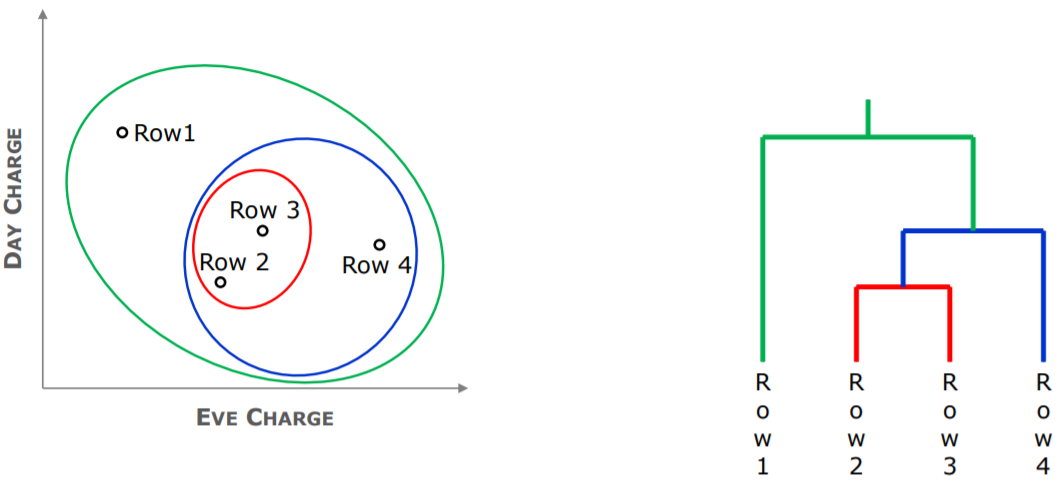
\includegraphics[height=0.25 \linewidth]{clustering/pict/cluster_aggl.png}
	\caption{Clustering gerarchico sotto forma di dendrogramma}
\end{figure}

Di seguito un rapido riassunto dei passaggi dell'algoritmo:

\begin{enumerate}
	\item Calcolare la matrice di prossimità (se necessario).
	\item \textbf{Ripeti:}
	\begin{itemize}
		\item Unione di due cluster vicini.
		\item Aggiorna la matrice di prossimità (o delle distanze) che riflette la prossimità tra il nuovo cluster e il cluster originale		.
	\end{itemize}
	\item \textbf{Finché} rimane un solo cluster.
\end{enumerate}

Si pone ora il problema di calcolare la prossimità tra due cluster . Ci sono in particolare tre modi:
\begin{itemize}
	\item  \textit{Min or Single Linkage}: minore distanza tra tutte le possibili coppie di elementi presenti nei due cluster, per come è definita è ovviamente la soluzione più ottimista.
	\item \textit{Max or Complete Linkage}: maggiore distanza tra tutte le possibili coppie di elementi presenti nei due cluster, è una soluzione più robusta o pessimista.
	\item \textit{Group Avarage or Avarage Linkage}: media distanza tra tutte le possibili coppie di elementi presenti nei due cluster, è una soluzione abbastanza usata in quanto media le distanze.
	\item \textit{metodo di Ward}: assume che i cluster siano rappresentati dai centroidi. Misura la prossimità tra due cluster come l'incremento della somma di scarti quadratici che risulta dalla fusione di due cluster.
\end{itemize}
	\begin{figure}[H]
	\begin{minipage}[b]{0.3\linewidth}
		\centering
		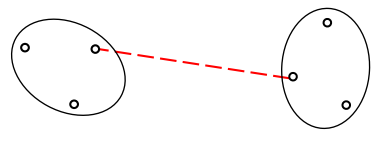
\includegraphics[width=\linewidth]{clustering/pict/sing_linkage.png}
		\caption{ \textit{Single}}
	\end{minipage}
	\hfill
	\begin{minipage}[b]{0.3\linewidth}
		\centering
		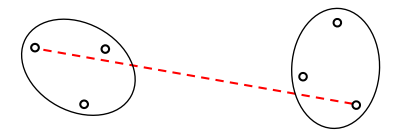
\includegraphics[width=\linewidth]{clustering/pict/complete_linkage.png}
		\caption{\textit{Complete}}
	\end{minipage}
	\begin{minipage}[b]{0.3\linewidth}
	\centering
	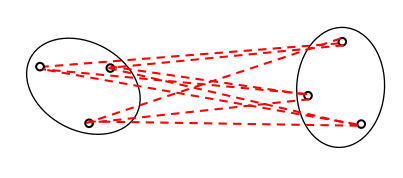
\includegraphics[width=\linewidth]{clustering/pict/average_linkage.png}
	\caption{\textit{Average}}
\end{minipage}
\end{figure}

Le \textbf{caratteristiche} chiave di questi algoritmi sono le seguenti:
\begin{itemize}
	\item \textit{Mancanza di una funzione globale di oggetto:} per questo motivo non può risolvere problemi di ottimizzazione globale.
	\item \textit{Abilità di gestire cluster di diverse dimensioni:} può gestire cluster con dimensioni differenti, i cluster possono anche essere pesati o meno.
	\item \textit{Le decisioni di unione sono definitive:} non si può tornare indietro rispetto alla decisione (approccio greedy).
\end{itemize}

Le \textbf{problematiche} più importanti sono invece:
\begin{itemize}
	\item Computazionalmente molto pesante e richiede molto spazio.
	\item Decisioni di unione di cluster sono sub-ottimali quindi creano rumore soprattutto per dati documentali. 
\end{itemize}

\subsubsection{Density-Based Clustering}
Di seguito la descrizione della classe di algoritmi basati sulla densità. In particolare le tecniche di clustering basate sulla densità si occupano di \textit{trovare regioni con un'alta densità di oggetti circondati da regioni con una bassa densità di oggetti.}
Passiamo ora a parlare di un algoritmo specifico, il \textit{DBSCAN.}

\paragraph{DBSCAN} E' un semplice ma efficace  algoritmo density-based che mostra un gran numero di concetti fondamentali tipici dell'approccio density-based. Ci sono diversi metodi per definire la densità, in particolare noi descriviamo il metodo center-based.
\begin{defn}
	Si definisce \textbf{densità} il numero di oggetti presenti all'interno di un raggio fissato ($\epsilon$) rispetto ad un oggetto.
\end{defn} 

Come facilmente intuibile la densità può variare fortemente al variare del raggio.
\begin{figure}[H]
	\centering
	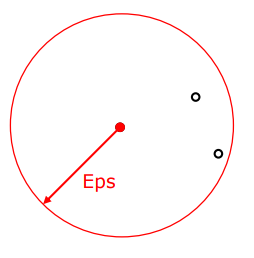
\includegraphics[height=0.25 \linewidth]{clustering/pict/density.png}
	\caption{Densità rappresentata graficamente}
\end{figure}

Definita la densità in questo modo, i punti vengono classificati in tre tipologie diverse:
\begin{itemize}
	\item \textit{Core point}: stanno all'interno della regione ad elevata densità. In particolare, un punto viene definito così se il numero di punti nel suo vicinato eccede un certo valore di soglia (MinPts) pre-impostato dall'utente. 
	\item \textit{Border point} : un punto che include nel suo vicinato un core point, quindi lui si considera un vicino di core point.
	\item \textit{Noise point}: non è né un core point né un border point.
\end{itemize}

Come negli altri casi di seguito i passaggi dell'algoritmo in maniera schematica:
\begin{enumerate}
	\item Etichettare tutti i core, border, noise point.
	\item Eliminare i noise point.
	\item Collegare con un ponte tutti i core point che sono all'interno dei rispettivi Eps.
	\item Trasformare ogni gruppo di core point connessi in cluster separati.
	\item Assegnare  ciascun border point al cluster associato al core point più prossimo.
\end{enumerate}

Come detto in precedenza la scelta dei parametri \textit{MinPts} e \textit{Eps} è fondamentale in quanto impatta fortemente sull'esecuzione di tutto l'algoritmo. Di seguito, invece,  quali sono le \textbf{differenze} principali tra l'algoritmo DBSCAN e l'algoritmo K-means:
\begin{itemize}
	\item DBSCAN e K-Means assegnano gli oggetti ad un singolo cluster, l'algoritmo delle k-medie però assegna tutti gli oggetti mentre il DBSCAN può omettere il rumore.
	\item DBSCAN può trattare cluster di diverse dimensioni e forme e non è affetto da rumori o outliers. K-medie hanno difficoltà con i cluster non globulari oppure di forme diverse. Entrambi gli algoritmi performano male quando i cluster hanno significative differenze di densità.
	\item L'algoritmo delle K-medie può essere usato per dato che hanno centroidi ben definiti come la media o la mediana. L'algoritmo DBSCAN invece richiede una definizione di densità che è basata sulla nozione tradizionale di distanza Euclidea.
	\item L'algoritmo delle K-medie può essere applicato a dati sparsi e a multi-dimensionali come ad esempio i dati documentali. Il DBSCAN in questi casi invece non performa per niente bene in quanto la definizione di densità Euclidea non funziona bene per dati multi-dimensionali.
	\item DBSCAN non fa assunzioni riguardo la distribuzione dei dati. L'algoritmo delle K-medie invece è equivalente ad approccio statistico di clustering che assume che tutti i cluster vengono da una distribuzione Gaussiana sferica con diverse medie ma con la stessa matrice di covarianza.
	\item Entrambi gli algoritmi cercano di costruire cluster utilizzando tutti gli attributi, ciò implica che non cercano cluster che riguardano solo un sottoinsieme degli attributi.
	\item L'algoritmo delle K-medie può trovare cluster che non sono ben separati, l'algoritmo di cluster invece mette insieme quelli sovrapposti.
	
	\item L'algoritmo delle K-medie ha complessità O(m) mentre il DBSCAN ha complessità O($m^{2}$) eccetto per i dati a poche dimensioni.
	\item DBSCAN produce lo stesso insieme di cluster dalla prima riproduzione mentre l'algoritmo delle k-medie tipicamente non lo fa quando i centroidi sono inizializzati casualmente. 
	\item DBSCAN determina automaticamente il numero di cluster mentre nell'algoritmo delle k-medie esso deve essere esplicitato in principio come parametro.
\end{itemize}

Vi sono altri algoritmi di density-based che non verranno trattati in questo momento quali: \textit{grid-based clustering}, \textit{subspace clustering}, \textit{kernel density function}.

\subsubsection{Graph-based Clustering Algorithm}
Gli algoritmi di clustering gerarchico usano una visione dei dati basata sui \textit{grafi,} in cui i dati sono rappresentati come \textit{nodi} e la prossimità tra due istanze è rappresentata dal peso del \textit{ponte} che c'è tra i rispettivi nodi. Sono stati esplorati algoritmi di clustering graph-based che esplorano diverse caratteristiche e proprietà dei grafi. Gli approcci chiave sono i seguenti:
\begin{itemize}
	\item \textit{Sparsificare il grafo di prossimità:} tagliare, rimuovere certi archi che non superano la verifica di una certa condizione. (Es. tutti gli archi che non superano una certa soglia, oppure un concetto di vicinato). 
	\item\textit{Definire una misura di similarità:} tra due oggetti basati sul numero di oggetti vicini che condividono. Questo approccio aiuta a diminuire i problemi che nascono con cluster di dimensioni diverse e con densità diverse. 
	\item \textit{Definire oggetti core e costruire cluster attorno ad essi:} Necessita l'introduzione di grafo di prossimità density-based.
	\item \textit{Utilizzare l'informazione nel grafo di prossimità} per fornire una maggiore valutazione per cui due cluster dovrebbero essere uniti. 
\end{itemize}

\begin{figure}[H]
	\centering
	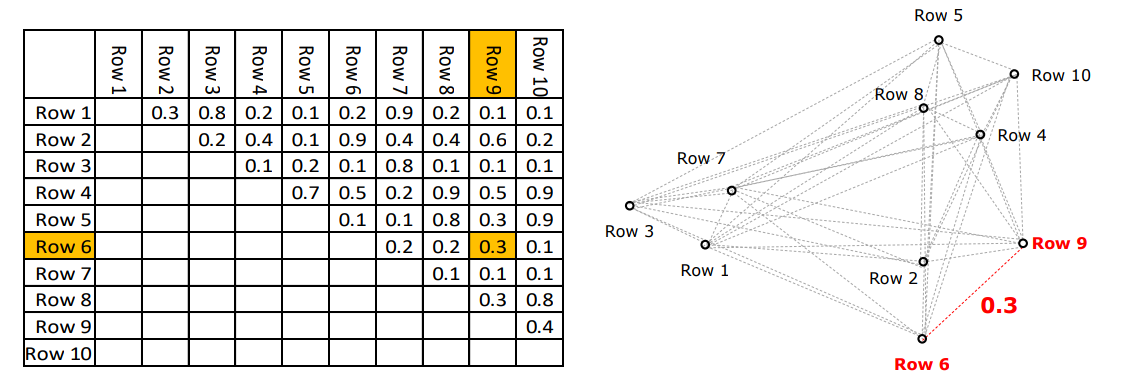
\includegraphics[height=0.30 \linewidth]{clustering/pict/proximity_graph.png}
	\caption{Correlazione tra matrice di prossimità e grafo di prossimità.}
\end{figure}

Come si può notare, ogni oggetto a un certo livello di similarità con \textit{ogni} altro oggetto, per la maggior parte del dataset gli oggetti sono molto più simili ad un basso numero di oggetti e molto poco simili ad un alto numero di oggetti. Un 'operazione utile è quella di sparsificare il grafo/matrice di prossimità ossia di settare alcuni dei valori di prossimità molto bassi a 0. Il "molto bassi" viene identificato da un valore soglia. Questo serve a \textit{rompere tutti i nodi che hanno una prossimità sotto una data soglia o a tenere solo i collegamenti ai k-nearest neighbours per ogni punto}

\begin{defn}
	Definiamo quindi il \textbf{K-Nearest Neighbour} il numero di valori di archi che prendo come vicinato per ogni riga della matrice.
\end{defn}
Come facilmente intuibile ci sono diversi vantaggi nello sparsificare la matrice. In primo luogo \textit{la riduzione della dimensione dei dati,} settare dei valori a 0 infatti implica la non considerazione di quei collegamenti nell'algoritmo. In secondo luogo \textit{ l'algoritmo di clustering potrebbe lavorare meglio,} questo perché la sparsificazione potrebbe eliminare degli outlier  o quegli elementi che costituiscono soltanto del rumore. Un ultimo motivo altrettanto importante è che \textit{si possono trovare anche partizioni interessanti di quel grafo.}

La sparsificazione deve essere vista come lo step preliminare prima dell'uso dell'algoritmo di clustering. \textit{Raramente succede però che la sparsificazione splitti la matrice in componenti connesse ognuna corrispondente ad un dato cluster.} L'idea è quella di ripetere ciclicamente la sparsificazione fino ad ottenere dei grafi partizionati ben definiti. Sono stati sviluppati in letteratura diversi tipi di algoritmi di cluster graph-based e che rispondono a queste necessità.

\paragraph{Minimum spanning tree (MST)} L'algoritmo inizia con l'albero di supporto o a costo minimo (minimum spanning tree) del grafo di prossimità e può essere visto come un'applicazione della sparsificazione per trovare i cluster. In particolare:
\begin{defn}
	Si definisce  \textbf{albero di supporto a costo minimo} di un grafo un sottografo che rispetta le seguenti caratteristiche:
	\begin{itemize}
		\item Non ha cicli, o equivalentemente è un albero.
		\item Contiene tutti i nodi del grafo.
		\item Ha il minimo costo totale dei pesi associati ai suoi alberi di tutti i possibili spanning tree.
	\end{itemize}
\end{defn}

Quando si parla di albero di supporto si assume che funzioni solo con le distanze o le dissimilarità.
\begin{figure}[H]
	\centering
	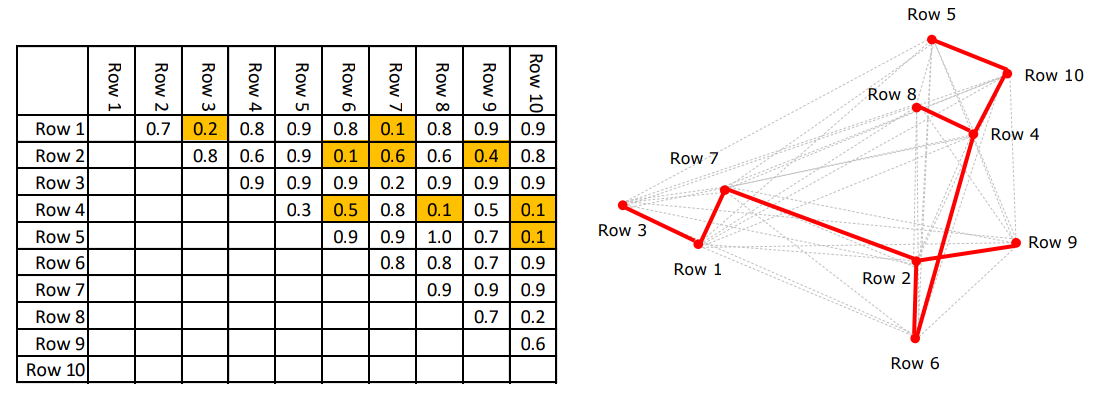
\includegraphics[height=0.30 \linewidth]{clustering/pict/mst.png}
	\caption{Albero di supporto con relativa matrice.}
\end{figure}
L'algoritmo di costruzione è il seguente:
\begin{enumerate}
	\item Calcolare il MST per grafo di dissimilarità.
	\item \textbf{Ripetere}
	\begin{itemize}
		\item Creare un nuovo cluster per rompere il collegamento corrispondente alla più grande dissimilarità.
		\item \textbf{Finché} rimangono solo cluster singoli.
	\end{itemize}
	
\end{enumerate}

\paragraph{Opossum} è un algoritmo disegnato appositamente per clusterizzare dati multidimensionali e sparsi come i dati documentali o tipo il cestino della spesa. Si basa sullo stesso principio, ossia sulla sparsificazione del grafo. L'algoritmo nello specifico è il seguente:
\begin{enumerate}
	\item Calcola il grafo di similarità sparsificato.
	\item Partiziona il grafo in k componenti distinte (cluster) usando METIS.
\end{enumerate}
Come notiamo, la misura di similarità deve essere appropriata rispetto al tipo di dati che stiamo trattando. come ad esempio la misura di Jaccard o quella del coseno.  \`E un algoritmo molto veloce e semplice e tende a partizionare i dati in cluster di egual dimensione.

\paragraph{Chamaleon} \`E un algoritmo di clustering agglomerativo che combina \textit{un iniziale partizionamento dei dati}, con un ulteriore schema di clustering gerarchico che usa la nozione di \textit{vicinanza e interconnettività.} L'idea chiave è che \textit{due cluster devono essere uniti solo se il cluster risultante è simile ai cluster di partenza.}
L'algoritmo  si articola nei seguenti passaggi:
\begin{enumerate}
	\item Costruire un grafo k-nearest neighbour.
	\item Partizionare il grafo usando un algoritmo di partizionamento a multi livelli.
	\item \textbf{Ripetere}
	\begin{itemize}
		\item Unire i cluster che preservano maggiormente la somiglianza rispetto alla relativa vicinanza e interconnettività..
		\item \textbf{Finché} non possono essere uniti ulteriori cluster.
	\end{itemize}
	
\end{enumerate}

Questo algoritmo riesce a clusterizzare dati spaziali considerando anche il rumore e gli outlier, riesce, inoltre, a gestire anche cluster di diversa forma e di diversa densità. Questo algoritmo ha però problemi \textit{quando il processo di partizionamento non subisce la creazione di sotto cluster.}
\begin{figure}[H]
	\centering
	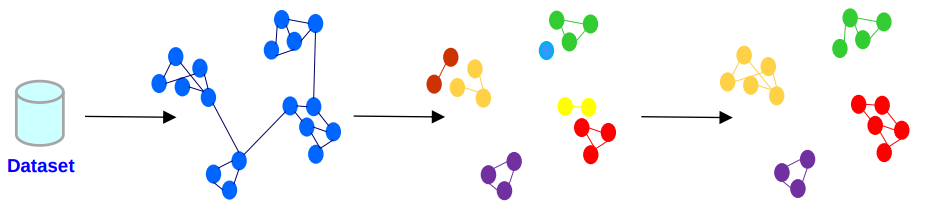
\includegraphics[height=0.18 \linewidth]{clustering/pict/chamaleon.png}
	\caption{Schema di funzionamento dell'algoritmo Chamaleon.}
\end{figure}

\subsection{Clustering Evaluation(*)}
La trattazione è sempre la solita, è presente un problema di clustering da risolvere. Quando si risolve un problema di questo tipo l'efficienza di un algoritmo di clustering viene valutata tramite:
\begin{itemize}
	\item Similarità.
	\item Esclusività dei cluster o misure fuzzy di sovrapposizione.
	\item Se i cluster sono completi o parziali.
\end{itemize}

Si decide di impostare un piano sperimentale, si selezionano successivamente un certo numero di algoritmi di clustering e ai testano per vedere quali funzionano meglio. L'obiettivo è avere quindi gli stessi metodi dei classificatori per capire quando un algoritmo di clustering possa essere considerato migliore di un altro. Purtroppo il concetto di clustering è molto più complesso visto che non si conoscono esattamente il risultato da ottenere.
Le \textbf{problematiche} più grosse nella valutazione sono:
\begin{itemize}
	\item Determinare la tendenza dei cluster (che non siano fatti a caso).
	\item Determinare il numero corretto di cluster (qualunque cosa significhi).
\end{itemize} 
Si utilizzano tre diversi tipi di indici che servono a validare i nostri cluster:
\begin{itemize}
	\item \textit{Esterni o supervisionati}: misurano l'estensione per cui la struttura di clustering trovata combaci con qualche struttura esterna (presupponendo di avere una vaga idea di come i dati dovrebbero organizzarsi).
	\item \textit{Interni o non supervisionati}: misurano la bontà di una struttura di clustering senza tener conto di informazioni esterne. In particolare, essi possono essere:
	\begin{itemize}
		\item Misure di coesione: determinano la connessione tra elementi di un cluster
		\item misure di separazione: quanto sono ben distiniti i cluster. 
	\end{itemize}
	\item \textit{Relativi}: comparano differenti algoritmi di clustering. 
\end{itemize}
\subsubsection{Esterni o supervisionati(*)}

Si supponga di avere un partizionamento $P = \{P_{1}, ..., P_{R}\}$ di R insiemi disgiunti con $m$ elementi. 

Sia ora: $C = \{C_{1}, ..., C_{K}\}$, la partizione ottenuta con un algoritmo di clustering in $K$ cluster. Si compari il partizionamento P con C per vedere quali siano i casi che si realizzano.
Ci sono ovviamente quattro casi che possono verificarsi:
\begin{enumerate}
	\item[a.]  x e y appartengono allo \underline{stesso} cluster di C e alla \underline{stessa} categoria di P
	\item [b.] x e y appartengono allo \underline{stesso} cluster di C e a \textit{diverse} categorie di P
	\item [c.] x e y appartengono a \textit{diversi} cluster di C e alla \underline{stessa} categoria di P
	\item[d.]  x e y appartengono a \textit{diversi} cluster di C e a \textit{diverse} categorie di P
\end{enumerate}
Ovviamente le coppie che possiamo formare sono:

\[M =  \frac{m(m-1)}{2} =  a+b+c+d\]

\begin{figure}[H]
	\centering
	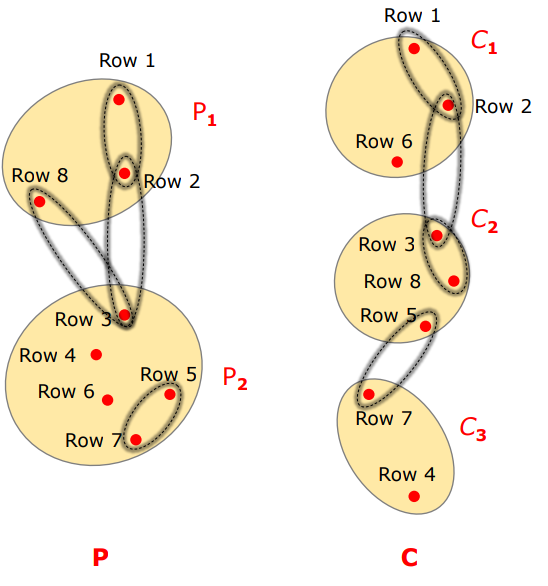
\includegraphics[height=0.40 \linewidth]{clustering/pict/partizionamenti.png}
	\caption{Partizionamenti C e P e formazione delle coppie.}
\end{figure}

Si definiscono di seguito diverse misure di similarità:

	 \begin{defn}
		Si definisce \textbf{Rand} il seguente indice:
		 \[R = \frac{a + d}{M} \quad R \in [0,1]\]
			\end{defn}
		\begin{defn}
			Si definisce \textbf{Jaccard} il seguente indice:
			\[J = \frac{a}{a + b + c} \quad J \in [0,1]\]
		\end{defn}
		\begin{defn}
			Si definisce \textbf{Fowlkes and Mallows} il seguente indice:
			\[FM = \sqrt{\frac{a}{a + b} \times \frac{a}{a + c}} \quad FM \in [0,1]\]
		\end{defn}
		 \begin{defn}
			Si definisce \textbf{$\Gamma$ statistics} il seguente indice:
			\[\Gamma = \frac{M \times a - (a+b)\times (a+c)}{\sqrt{(a+b)\times (a+c)\times(M-a-b)\times(M-a-c)}} \quad \Gamma \in [-1,1]\]
		\end{defn}	
Per come sono definiti, più è grande il valore che assumono questi indici più sono simili C e P.
\subsubsection{Interni o non supervisionati(*)}
Diversi indici di interni di validità del partizionamento dei cluster si basano sulla \textit{coesione} e sulla \textit{separazione}. L' idea è quella di ottenere un valore di coesione alto e un valore di separazione basso.
In generale, \textit{si valuta la validità totale di un cluster fatto da un insieme di K cluster come la media pesata delle validità di ogni singolo cluster.}

\[ overall\_validity = \sum_{i = 1}^{K}w_{i} \cdot validity(C_{i})\]
In cui la validità può essere la coesione, la separazione o una combinazione lineare di queste; i pesi invece variano in base alla misura di validità del clustering.
Supponendo di avere dei cluster basati su grafi si può definire la coesione e la separazine in questo modo:

\begin{defn}
	Si definisce \textbf{coesione} la somma dei pesi dei ponti nel grafo di prossimità che connettono i punti all'interno del  cluster.
	\[ cohesion(C_i) = \sum_{x, y \in C_i} proximity(x,y) = \sum_{x y \in C_i} similarity(x,y)\]
\end{defn}
Per questo motivo la coesione e la similarità sono massimizzate quando vengono minimizzate la dissimilarità/distanza.

\begin{defn}
	Si definisce \textbf{separazione} la somma dei pesi dei ponti nel grafo di prossimità che connettono i punti di un cluster ai punti di un altro cluster.
	\[separation(C_{i}, C_{j}) = \sum_{x \in C_{i},y\in C_{j} }proximity(x,y) = \sum_{x \in C_{i},y\in C_{j} }similarity(x,y)   \]
\end{defn}
Per gli algoritmi di clustering basati sui prototipi invece le definizioni cambiano un pochino:
\begin{defn}
	Si definisce \textbf{coesione} la somma delle prossimità rispetto al prototipo all'interno del  cluster.
	\[ cohesion(C_i) = \sum_{x \in C_i} proximity(x, c_i) = \sum_{x\in C_i} similarity(x, c_i)\]
\end{defn}
\begin{defn}
	Si definisce \textbf{separazione} la prossimità tra due prototipi di due cluster diversi.
	\[separation(C_{i}, C_{j}) = proximity(c_{i}, c_{j}) = similarity(c_{i}, c_{j})   \]
\end{defn}
E' molto difficile dare una definizione sempre uguale dei pesi da fornire ai vari cluster nel momento in cui si vuole operare una misura di validità, per semplificare il problema bisogna fare riferimento alla seguente tabella.
\begin{figure}[H]
	\centering
	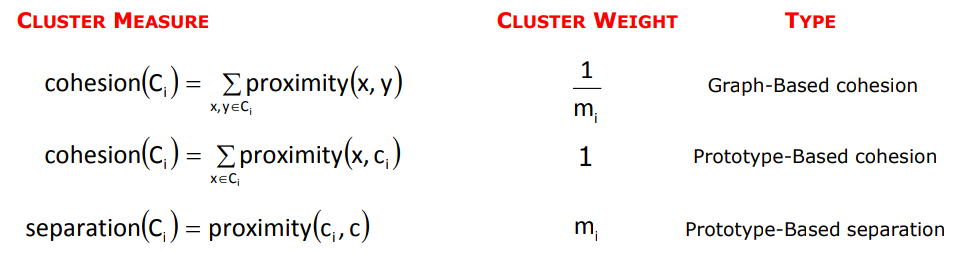
\includegraphics[height=0.250 \linewidth]{clustering/pict/pesi_validity.png}
	\caption{Pesi da usare a seconda del tipo di algoritmo di clustering.}
\end{figure}
Durante questa trattazione ci si è concentrati sulle misure di coesione e di separazione come valutazione totale di un gruppo di cluster; diverse di queste misure possono essere anche applicate per valutare i singoli cluster. L' obiettivo è \textit{ordinare i cluster secondo il loro specifico valore di validità;} in particolare, un cluster con un alto valore di coesione deve essere considerato migliore rispetto ad un cluster con un basso valore di coesione.
Se sono presenti cluster non molto coesi potrebbe risultare utile separarli in dei cluster più fortemente coesi. Allo stesso modo se due cluster sono relativamente coesi ma non troppo ben separati potrebbe essere utile provare ad unirli.

\textit{Risulta quindi utile valutare un oggetto all'interno del cluster secondo la misura in cui quell'oggetto contribuisce alla coesione o alla separazione.} Graficamente si otterrebbe che gli oggetti che si trovano più "all'interno" del cluster dovrebbero contribuire in modo maggiore alla coesione, mentre quelli più esterni avranno un contributo minore. Proprio per questo motivo si definisce l'indice di Silhouette che combina coesione e separazione per l'i-esimo oggetto all'interno del cluster.
\begin{defn}
	Si definisce \textbf{coefficiente di Silhouette} per l'i-esimo oggetto all'interno di un cluster la seguente espressione:
	\[s_i = \frac{b_i - a_i}{max(a_i,b_i)} \in [-1,+1]\]
\end{defn}

Dove:
\begin{itemize}
	\item $a_{i}$ è la distanza media dell'oggetto i-esimo rispetto a tutti gli oggetti del cluster a cui appartiene.
	\item $b_{i}$ è il minimo delle distanze medie dell'oggetto i-esimo da tutti gli oggetti degli altri cluster.
\end{itemize}

\textit{Valori negativi} di questo coefficiente significano che la distanza media dei punti nello stesso cluster è maggiore della distanza media minima di quei punti rispetto ai punti di un altro cluster.  Per come è definito sono preferibili \textit{valori positivi} poiché il coefficiente assume il valore 1 quando $a_i = 0$.

Si possono, quindi, calcolare il \textit{Coefficiente medio di silhouette} semplicemente calcolando la media dei coefficienti dei punti di un dato cluster. Una misura totale della bontà di un clustering può quindi essere il coefficiente medio di silhouette calcolato su tutti i punti.
Per quanto riguarda il clustering gerarchico, non si usa il coefficiente di silhouette ma il \textbf{Cophenetic Correlation Coefficient.}

Questo coefficiente misura il grado di similarità tra la matrice di prossimità (P) e la matrice Cophenetic (Q) i cui elementi registrano il livello di prossimità tra coppie di osservazioni raggruppate all'interno dello stesso cluster.
 Il valore varia da $[-1,1]$. Più il valore è vicino a 1 meglio l'algoritmo gerarchico si adatta ai nostri dati.
 \subsubsection{Paradigma di validità(*)}

 Sia gli indici interni che quelli esterni sono strettamente correlati ai metodi statistici, in particolare ai test di ipotesi. Il paradigma di validità è un processo schematico che ci porta a dire se ci sia struttura o meno nei nostri dati e si articola nel seguente modo:
 
 \paragraph{Identificare la struttura e il tipo di validazione} La struttura della ricerca è basata sulla seguente ipotesi nulla:
 \textbf{Non c'è struttura nel dataset.}
 \paragraph{Determinare un indice di validazione} Cercare quale sia l'indice di validazione più appropriato per lo schema di clustering.
 \paragraph{Definire un'ipotesi nulla di non struttura} Il tipo di ipotesi che si va a fare dipende dal tipo di problema, può essere ad esempio :
 \begin{itemize}
 	\item \textit{Random Position} (i records si distribuiscono casualmente nello spazio n-dimensionale dei record). Viene usata per i dati razionali.
 	\item \textit{Random Graph } non  interessa la posizione ma che ci sia una certa struttura di similarità. Viene usata per prossimità ordinali tra coppie di dati.
 	\item \textit{Random Label}: etichettare le osservazioni in modi differenti non cambia il tipo di coerenza che ottengo nel mio esperimento. Viene usata per tutti i tipi di dati.
 \end{itemize}
\paragraph{Stabilire le fondamenta della distribuzione sotto l'ipotesi nulla} Può essere operata un'analisi Monte Carlo e BootStrapping.
\paragraph{Calcolare gli indici} Si calcolano tutti gli indici visti in precedenza.
\paragraph{Testare l'ipotesi nulla} Si vuole arrivare ovviamente a rigettare l'ipotesi nulla. Questo rigetto non implica che ci sia necessariamente struttura nei dati ma implica che sicuramente non c'è non-struttura. 
 
 \subsubsection{Selezione del numero di cluster(*)}
 Ha senso porsi il problema di scegliere il numero di cluster solo dopo che l'analisi precedente ha permesso di dedurre che è presente struttura adatta per un'analisi di clustering. In particolare, si utilizzano i \textit{criteri relativi} che sono criteri che si concentrano sul confronto dei diversi risultati generati dai diversi algoritmi di clustering oppure sui risultati diversi prodotti dallo stesso algoritmo di clustering ma con parametri di input differenti.
 Gli indici principali per calcolare il numero di cluster sono:
 \begin{itemize}
 	\item \textit{Calinski and Harabasz:} Il valore di K corrispondente al massimo è preso per essere l'ottimale numero di cluster.
 	\item \textit{Dunn:} Il valore di K corrispondente al massimo è preso per essere l'ottimale numero di cluster.
 	\item \textit{Devies-Bouldin:} Il valore di K corrispondente al minimo è preso per essere l'ottimale numero di cluster.
 \end{itemize}
 
Gli indici per gli algoritmi di cluster basati sulle misture probabilistiche sono invece:
 \begin{itemize}
 	\item \textit{Akaike Information Criterion (AIC):} Il valore di K corrispondente al minimo è preso per essere l'ottimale numero di cluster.
 	\item \textit{Minimum Description Length (MDL):} Il valore di K corrispondente al minimo è preso per essere l'ottimale numero di cluster.
 	\item \textit{Bayesian Information Criterion (BIC):}Il valore di K corrispondente al minimo è preso per essere l'ottimale numero di cluster.
 \end{itemize}
 
 Per un algoritmo di clustering che richiede come input un numero di cluster inserito dall'utente  si possono ottenere una sequenza di struttura di clustering iterando l'algoritmo di clustering $r$ volte dove $K$ spazia da $K_{min}$ a $K_{max}$.
 Di seguito ora  l'algoritmo che genera la sequenza delle strutture di clustering:
 \begin{itemize}
 	\item Scegliere un algoritmo di clustering e un indice di validazione.
 	\item \textbf{FOR $K_{min}$ to $K_{max}$:}
 	\begin{itemize}
 		\item \textbf{FOR $i = 1$ to $r$:}
 		\begin{itemize}
 			\item Lanciare l'algoritmo di clustering con k cluster e cambiare i parametri rispetto al lancio precedente.
 			\item Calcolare il valore $q$ dell'indice di validità e imporre $q(i) = q$
 		\end{itemize}
 		\item Scegliere il miglior valore $q^{*}$ tra ${q_1, q_2,...,q_r}$.
 		\item Imporre $Q(K) = q^{*}$.		 
 	\end{itemize}
 \end{itemize}
 
 \begin{figure}[H]
 	\centering
 	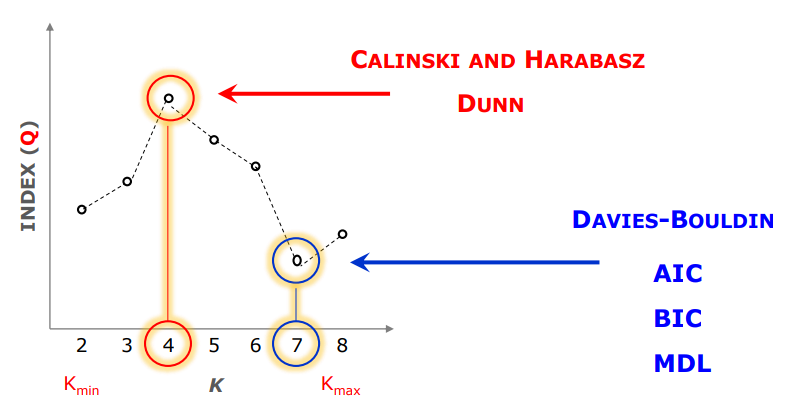
\includegraphics[width=0.7 \linewidth]{clustering/pict/cluster_validity.png}
 	\caption{Scelta del numero di cluster a seconda dell'indice.}
 \end{figure}

%

\section{Association Analysis}
\subsection{Introduction (*)}

L'analisi di associazione ci riporta al concetto di causalit\`a di variabili: dati certi valori di attributi cosa posso dire del valore di un altro attributo?

Le regole associative ci permettono di prendere delle scelte molto operative in diversi ambiti, in particolare in quello che viene chiamato \textit{market busket analysis}. 
Il problema del carrello tratta il posizionamento di prodotti in un negozio. Si sa che all'acquisto di un certo prodotto si tende a acquistare altri prodotti connessi, quindi si cercano queste associazioni basandosi sul carrello della spesa dei clienti (appunto market basket) per poi capire come impostare la disposizione sugli scaffali.

\textbf{Obiettivo}: identificare quali siano gli \textbf{item associati} per poter prendere delle decisioni. In sostanza si generano \textbf{Regole associative} formate da coppie di insiemi \textit{antecedente} e \textit{conseguente}.

es. \{Beer\} $\rightarrow$ \{swiss cheese\} 

\quad \{antecedente\} $\rightarrow$ \{conseguente\}\\
\textbf{NB}: non \`e una causalit\`a ma un'associazione

L'analisi si basa sullo studio di due diversi dataset:
\begin{itemize}
	\item Product set: contiene informazioni legate ai prodotti come il nome e il prezzo
	\item Transaction set: contiene informazioni legate agli acquisti dei clienti, ogni record corrisponde ai prodotti presenti nel carrello del cliente
\end{itemize}

Si organizza il dataset delle transazioni in formato binario, ovvero ogni colonna indica se in una data transazione un certo prodotto sia o meno presente.

\begin{figure}[H]
	\centering
	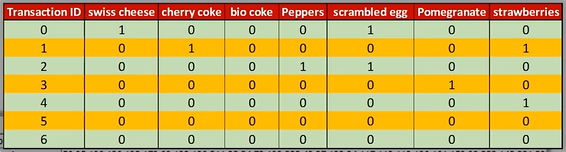
\includegraphics[height=0.25 \linewidth]{association/pict/transaction_set_bin.png}
	\caption{esempio: transaction set binarizzato}
\end{figure}
\clearpage
\noindent
Consideriamo:

$I = \{i_1, i_2,...,i_d\}$ il set di tutti gli item nel market basket

$T = \{t_1,t_2,...,t_N\}$ l'insieme di tutte le transazioni

\begin{defn}
	Una collezione di zero o più item è chiamata \textbf{Itemset}.
\end{defn} 
\begin{defn}
	Se un itemset contiene k item \`e detto \textbf{K-Itemset}.
\end{defn}
\begin{defn}
	L'itemset che non contiene alcun elemento è detto \textbf{empty set}.
\end{defn}
\begin{defn}
	La \textbf{transaction width} è il numero di item presenti in una transazione
\end{defn}
	 
Una transazione $t_j$ contiene l'itemset $X$, se $X$ è un sottoinsieme di $t_j$.

\begin{defn}
	Il \textbf{Support count} è il numero di transazioni che contentono uno specifico itemset.

\[ \sigma(X) = |\{t_i | X \subseteq t_i, t_i \in T\} \]
\end{defn}

\begin{defn}
Una \textbf{regola di associazione} viene rappresentata come:

$X \rightarrow Y$

dove $X$ e $Y$ sono itemset disgiunti ($X \cap Y = \emptyset$).
\end{defn}
Una regola viene valutata in termini di \textit{supporto} e di \textit{confidenza}.

\begin{defn}
	\textbf{Support} determina quanto spesso una regola sia applicabile dato un data set:
	
	\[s\{x \rightarrow Y\} = \frac{\sigma(X \cup Y)}{N}\]
\end{defn}
\begin{defn}
	\textbf{Confidence} determina quanto frequente Y \`e presente in una transazione che contiene X (si assume che l'universo sia rappresentato partendo da X):
	
	\[c\{x \rightarrow Y\} = \frac{\sigma(X \cup Y)}{\sigma(X)}\]
\end{defn}

\textbf{Es}. \\
$X = \{swiss cheese, cheddar\}$, $Y = \{diet coke\}$\\
Assumiamo che:
\begin{itemize}
	\item $\sigma(x) = 8$ (support count)
	\item $N = 20$ (numero di transazioni)
	\item $\sigma(x,y) = 6$ 
\end{itemize}
Allora il support e la confidence della regola $X \rightarrow Y$ sono:

\[s\{X \rightarrow Y\} = \frac{\sigma(X \cup Y)}{N} = \frac{6}{20} = 0.3\]

\[c\{x \rightarrow Y\} = \frac{\sigma(X \cup Y)}{\sigma(X)} = \frac{6}{8} = 0.75\]

Perch\`e utiliziamo il supporto:
\begin{itemize}
	\item se troppo basso potrebbe esserci un'associazione casuale
	\item potrebbe non valere la pena seguire associazioni che si applicano in modo poco significativo dal punto di vista dei profitti 
\end{itemize}
Supporto utilizzato per eliminare regole non desiderate e condivide interessanti propriet\`a che possono essere sfruttate per la ricerca di regole associative efficaci.

La confidenza \`e molto importante perch\`e misura l'affidabilità dell'inferenza e:
\begin{itemize}
	\item un alta confidenza significa che Y sar\`a molto presente in transazioni con X 
	\item si stima la probabilit\`a condizionata di Y dato X
\end{itemize}
\begin{defn}
\textbf{Association Rule Mining Problem} può essere formalmente definito come: dato un set di transazioni T, trovare tutte le regole con $support \ge minsup$ e $confidence \ge minconf$, dove $minsup$ e $minconf$ sono i threshold corrispondenti alle due misure.
\end{defn}

\textit{Approccio a forza bruta} di association rule non \`e molto praticabile in quanto i tempi di computazione aumentano in modo esponenziale: 

$R = 3^d - 2^{d+1} + 1$.

\begin{figure}[H]
	\centering
	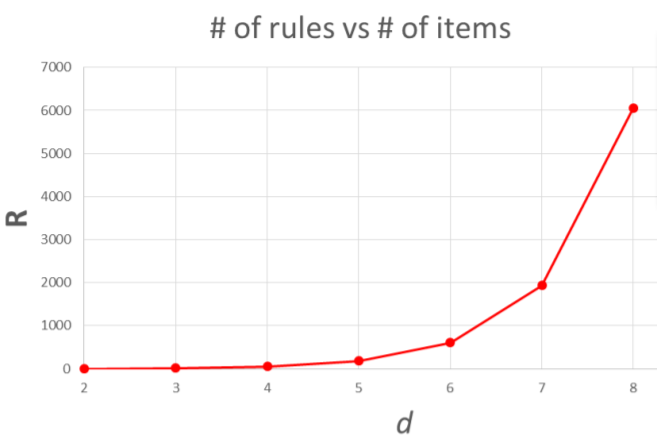
\includegraphics[height=0.4 \linewidth]{association/pict/brute_force.png}
	\caption{numero di regole calcolate in base al numero di itemset}
\end{figure}

Una strategia comunemente adottata in molti algoritmi \`e decomporre il problema in 2 grandi supertask:
\begin{itemize}
	\item\textit{Generazione dei frequenti itemset}: specifichiamo tutte e sole quelle regole per cui il supporto è maggiore del $minsup$, gli itemset generati sono chiamati \textbf{Frequent Itemset}
	\item \textit{Generazione delle regole}: estriamo tutte le regole con alta confidenza (maggiore di $minconf$) dai Frequent Itemset trovati precedentemente, queste regole vengono chiamate \textbf{Strong Rules}
\end{itemize}
\noindent
La complessità maggiore è richiesta dalla generazione dei Frequent Itemset.


\subsection{Rule Extraction}

Per comprendere l'inefficienza della generazione con l'approccio forza bruta pensiamo a questo esempio:
\begin{figure}[H]
	\hspace{-0.7 cm}
	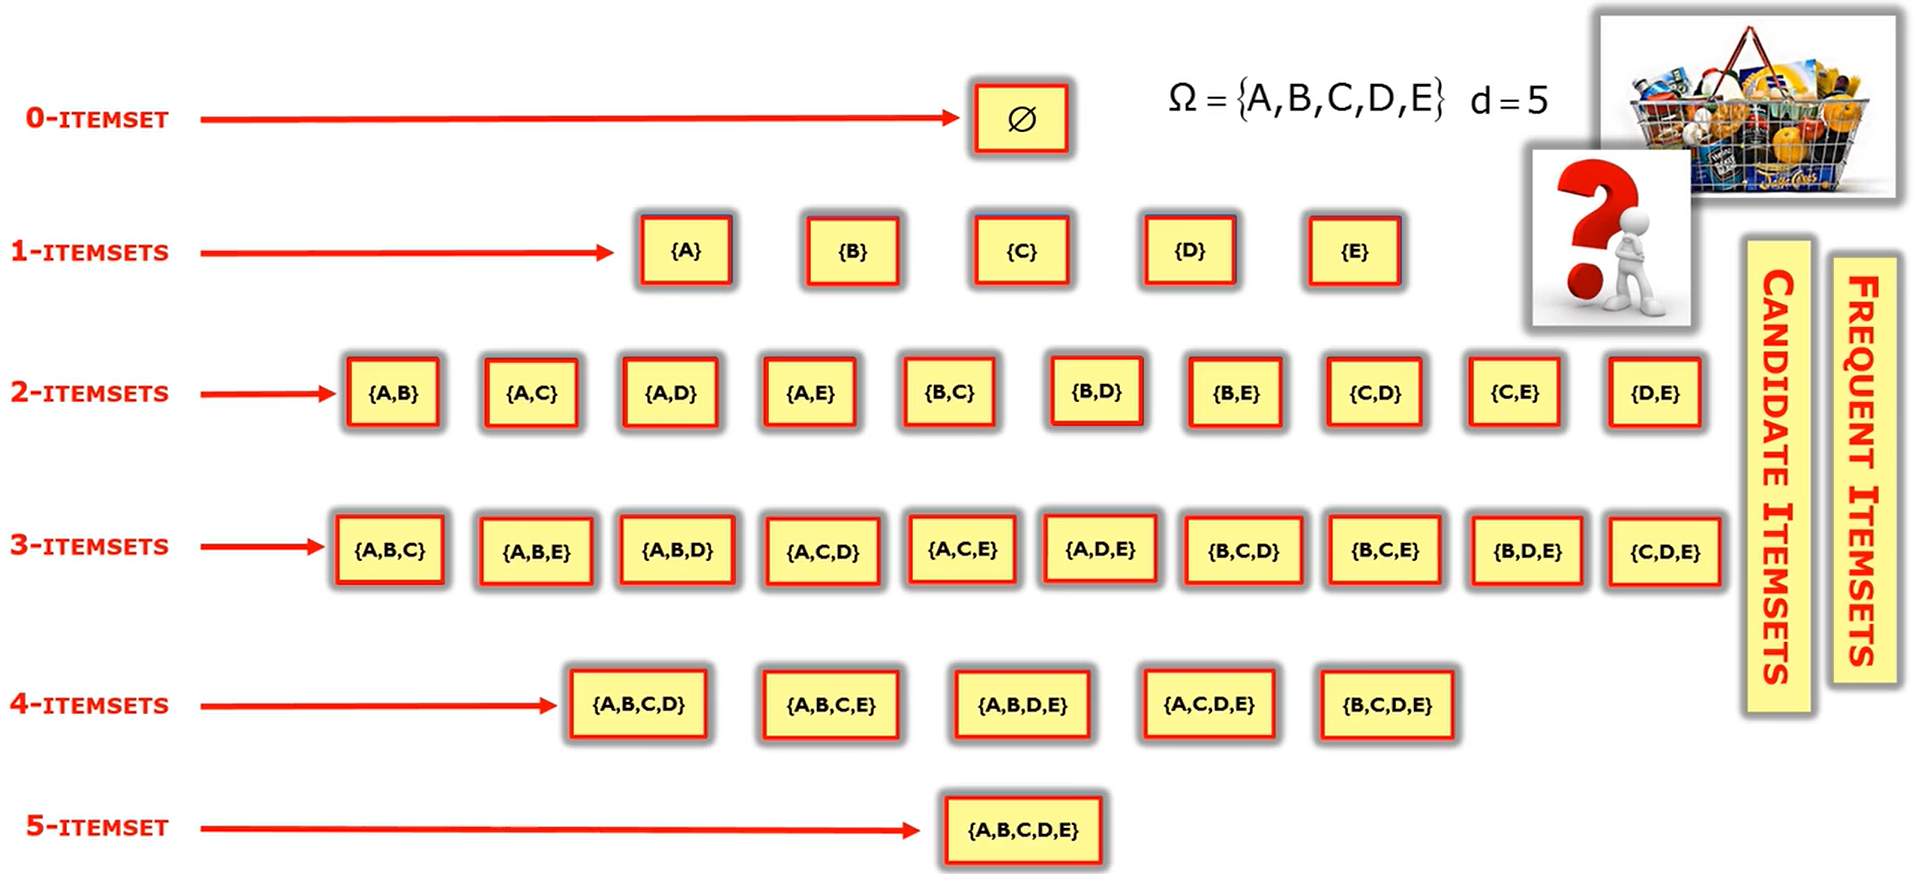
\includegraphics[height=0.5 \linewidth]{association/pict/k-itemset.png}
	\caption{k-itemset brute-force}
\end{figure}
\begin{defn}
	\textbf{Candidate Itemset}: l'insieme di tutti gli itemset che possiamo formare. Avranno un numero di item diverso. 
\end{defn}
Nel nostro caso il numero di itemset candidato è: $M = 2^{d} - 1 = 2^5 -1 = 31$

Come si può notare abbiamo un sistema a doppio cono che è tipica delle distribuzioni binomiali. Una volta che gli abbiamo considerati tutti ci interessano solo i più frequenti. \\
Se usassimo la forza bruta dovremmo calcolare per ogni itemset candidato il suo support count, e vedere se il suo supporto lo configura come un itemset frequente (molto dispendioso). 

I confronti da effettuare sono nell'ordine di $O(NMw)$, dove:
\begin{itemize}
	\item $N$ = numero di transazioni
	\item $M$ = numero di itemset candidato
	\item $w$ = massima lunghezza delle transazioni
\end{itemize} 

È decisamente troppo come numeri confronti contando che molti dei quali sono inutili o poco significativi.

Vi sono due approcci per ridurre il costo computazionale della generazione di itemset frequenti:
\begin{itemize}
	\item ridurre il numero di candidati itemset ($M$). Il principio Apriori \`e un metodo per eliminare alcuni candidati itemset senza contare il support count. 
	\item riduce il numero di confronti anzich\`e controllare tutte le possibili combinazioni, lo si fa con strutture dati avanzate
\end{itemize}

\paragraph{Principio Apriori} se un itemset \`e frequente, allora tutti i suoi sottoinsiemi sono frequenti.\\
Quindi se una regola ha una frequenza bassa allora tutte le regole che prevedono come sottoinsieme la stessa non supereranno quella frequenza pertanto \`e inutile considerarle. Si procede attraverso il \textbf{pruning} dell'albero delle sequenze per queste soluzioni, viene chiamato \textbf{support-based pruning} (vedi immagine).

\begin{figure}[H]
	\centering
	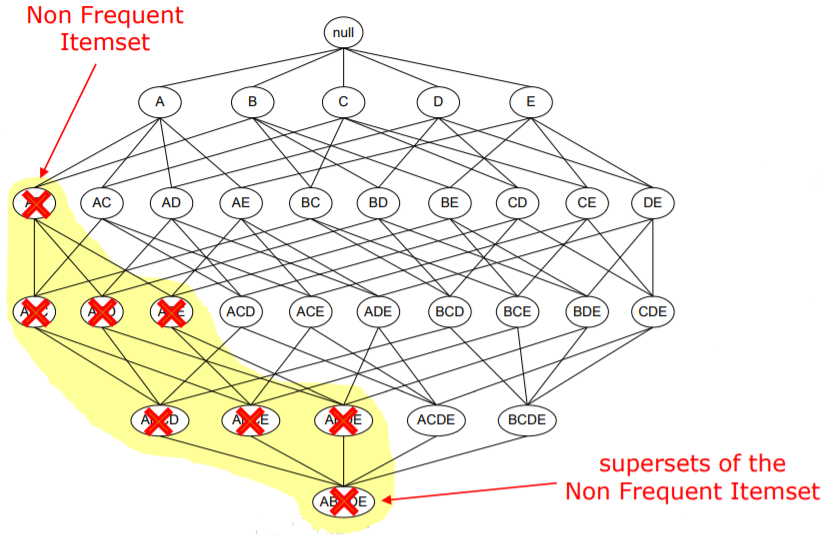
\includegraphics[height=0.5 \linewidth]{association/pict/pruning.png}
	\caption{esempio di support-based pruning}
\end{figure}

\subsubsection{Algoritmo apriori}
Genera due operazioni:
\begin{itemize}
	\item \textbf{Candidate Generation}: genera nuovi candidati k-itemset basati su (k-1)-itemset frequenti calcolati nella precedente iterazione
	\item \textbf{Candidate Pruning}: questa operazione elimina alcuni candidati k-itemset usando la strategia del support-based pruning
\end{itemize}

La complessit\`a computazionale soffre di 4 limiti:
\begin{itemize}
	\item \textit{Support threshold}: la soglia di supporto se troppo bassa non taglio molto l'albero, però non deve essere neanche troppo elevata altrimenti non considero associazioni rilevanti. 
	\item \textit{Numero di item (dimensionalit\`a)}: se il numero di item cresce, ci sar\`a bisogno di più spazio in memoria per registrare il support count degli item, inoltre bisogna considerare anche il costo dell'I/O per passare i dati.
	\item \textit{Numero di transazioni}: l'algoritmo scorre più volte tutta la lista di transazioni, pertanto un numero alto di transazioni inficia sui tempi.
	\item \textit{Avarage transaction width}: per dataset densi la lunghezza media delle transazioni tende ad essere grande. La massima lunghezza degli itemset frequenti tende ad aumentare quindi più sequenze candidato devono essere esaminate durante la generazione e support counting. In aggiunta aumenta il numero di archi traversi nell'albero durante il support counting.
\end{itemize}

\subsection{Maximal/Closed Frequent Itemsets}
\subsubsection{Rule Generation}
Ogni k-itemset frequente, Y pu\`o generare al limite $2^k-2$ regole di associazione. 

Una regola di associazione pu\`o essere estratta partizionando l'itemset Y in 2 sottoinsiemi non vuoti $\{X\}$ e $\{Y-X\}$, tale che $X \rightarrow Y -X$ soddisfa il threshold di confidenza.

\textbf{NB}: Tutte le regole generate da itemset frequenti sono esse stesse frequenti.

In pratica, il numero di itemset frequenti prodotti da transazioni possono essere molto grandi. È utile identificare itemset rappresentativi e piccoli con i quali derivare gli itemset grandi. Per questo si ragiona in due rappresentazioni:
\begin{enumerate}
	\item Maximal Frequent Itemset
	\item Closed Frequent Itemset
\end{enumerate}

\begin{defn}
	\textbf{Maximal Frequent Itemset} è definito come un Itemset Frequente per il quale nessuno dei suoi soprainsiemi immediati sono frequenti.
\end{defn}
\textbf{Maximal Frequent Itemset}: per ogni nodo si verifica il vincolo della frequenza e si definisce la frontiera dove un nodo non gode pi\`u di questa propriet\`a, corrisponde alla massima frontiera in cui mi posso spingere.

\begin{figure}[H]
	\centering
	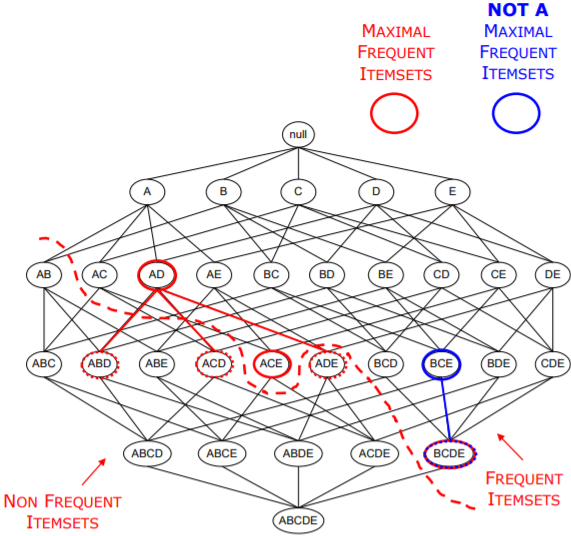
\includegraphics[height=0.7 \linewidth]{association/pict/max_freq_itemset.png}
	\caption{esempio di frontiera di maximal frequent itemset}
\end{figure}

\textbf{Nella pratica}: Un nodo \`e un Maximal Frequent Itemset se \`e frequente e se tutte le sue estensioni non sono frequenti.\\
\begin{itemize}
	\item Fornisce una rappresentazione compatta dell'insieme di itemset che cerchiamo, la pi\`u piccola espressione in cui gli itemset sono derivabili
	\item Calcolato dal più piccolo insieme di itemset dal quale tutti gli itemset frequenti possono essere derivati
	\item È praticabile solo l'algoritmo efficiente usato esplicita la ricerca dei maximal frequent itemset senza numerare tutti i suoi sottoinsiemi
\end{itemize}
Per costruzione \textit{per\`o} non ci dice quanto \`e il supporto rispetto ai suoi sottoinsiemi. In alcuni casi potrebbe servire avere una minima rappresentazione degli itemset frequenti che preservano l'informazione sul supporto.

\begin{defn}
	Un itemset X è \textbf{Closed Frequent Itemset} se nessun immediato superinsieme ha esattamente lo stesso support count di X. In ogni caso il suo spporto deve essere $\ge minsup$.
\end{defn}
Importante qunado vi sono gruppi di prodotti venduti a blocco ignorando gli altri.

\textbf{Es}
\begin{figure}[H]
	\centering
	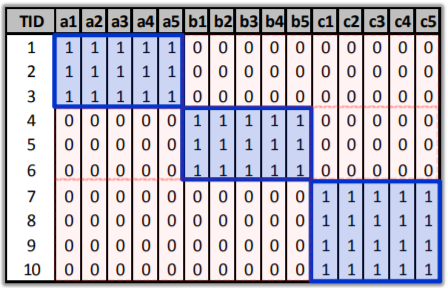
\includegraphics[height=0.5 \linewidth]{association/pict/close_freq_itemset.png}
	\caption{esempio di gruppi closed frequent itemset}
\end{figure}

Come si può notare in figura ogni gruppo di variabili (Gruppo A, B e C) è perfettamente associato e non hanno bisogno di mostrare items collegati ad altri gruppi. Assumendo che il $minsup = 20\%$, il numero totale di itemset frequenti è: $3 \cdot (2^5 -1) = 93$. In ogni caso vi sono solo 3 closed frequent itemset: 

$\{a1,a2,a3,a4,a5\}$

$\{b1,b2,b3,b4,b5\}$

$\{c1,c2,c3,c4,c5\}$


Questo tipo di itemset sono utili per rimuovere \textbf{regole di associazione ridondanti}. 
\begin{defn}
	Una regola di associazione $X \rightarrow Y$ \`e \textbf{ridondante} se esiste un'altra regola $X' \rightarrow Y'$ che rispetta certe propriet\`a. 
	\begin{itemize}
		\item $X \subseteq X'$
		\item $Y \subseteq Y'$
		\item $s(X \rightarrow Y)  = s(X' \rightarrow Y')$
		\item $c(X \rightarrow Y)  = c(X' \rightarrow Y')$
	\end{itemize}
\end{defn}

Mostriamo ora la gerarchia dei frequent itemset:
\begin{figure}[H]
	\centering
	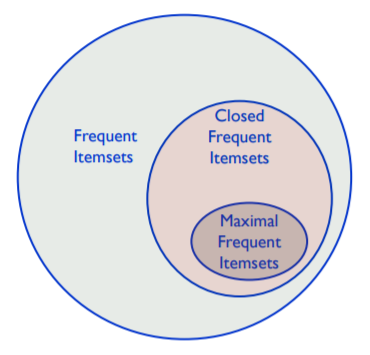
\includegraphics[height=0.45 \linewidth]{association/pict/itemset_freq.png}
	\caption{gerarchia dei frequent itemset}
\end{figure}

Come si può notare i Maximal Frequent Itemset sono inclusi nei Closed Frequent Itemset perchè nessun maxmal può avere lo stesso support count del suo immediato superset.

\subsection{Rules Evaluation (*)}
Generati gli insiemi di pattern potenzialmente utili, bisogna ordinarli in base al loro livello di attrattività per il dominio di applicazione. La valutazione della qualità viene effettuata seconodo due criteri:
\begin{itemize}
	\item \textbf{Statistical arguments}: per patterns di items indipendenti e coperti da poche transazioni. Il problema è che \textit{possono catturare relazioni spurie} nei dati, per evitare:
	\begin{itemize}
		\item \underline{Objective Interestingness Measure}: usare statistiche derivate dai dati per determinare quali pattern sono interessanti
		\item \underline{Supporto, confidenza e correlazione}
	\end{itemize}
	\item \textbf{Subjective arguments}: un pattern è considerato non interessante a meno che riveli informazioni inaspettate riguardo ai dati e alla conoscenza: \underline{es}. forte associazione tra acquisto di pannolini e birra. È difficile fare questo tipo di valutazioni, richiede una considerevole quantità di informazioni pregresse dagli esperti di domino.
\end{itemize}

Meglio cercare di applicare un approccio più \textit{oggettivo} alla valutazione: data-driven, indipendente dal dominio in cui si richiede un minimo input dagli utenti (solo dei threshold) e calcolato basandosi sulle frequenze calcolate in una \textbf{Contingency Table}.
\begin{figure}[H]
	\centering
	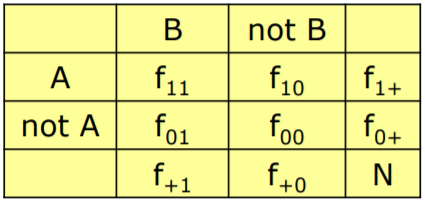
\includegraphics[height=0.2 \linewidth]{association/pict/contingency_table.png}
	\caption{contingency table}
\end{figure}
dove:
\begin{itemize}
	\item $f_{1+}$ = support count di A
	\item $f_{+1}$ = support count di B
	\item $N$ = nro di transazioni totali
\end{itemize}

Supponiamo che un direttore di un minimarket voglia analizzare la relazione tra le persone che bevono tè e persone che bevono caffè. La seguente contingency table è ottenuta considerando le transazioni disponibili:
\begin{figure}[H]
	\centering
	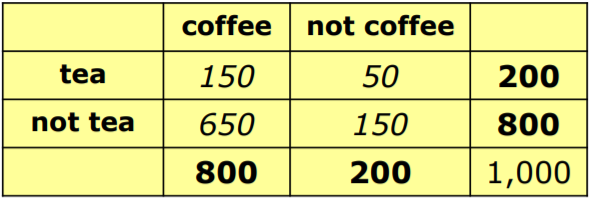
\includegraphics[height=0.2 \linewidth]{association/pict/contingency_table_es.png}
	\caption{contingency table}
\end{figure}

Ora valutiamo l'associazione: tea $\rightarrow$ coffee
\begin{itemize}
	\item $support = \frac{f_{11}}{N} = \frac{150}{1000} = 15\%$
	\item $confidence = \frac{f_{11}}{f_{1+}} = \frac{150}{200} = 75\%$
\end{itemize}

Ad una prima occhiata sembrerebbe che le persone che bevono tè tendono a bere anche caffè (vedi confidenza). Ma se notiamo le persone che bevono caffè, a prescindere dal tè sono l'$80\%$ ($\frac{800}{1000}$), mentre la frazione dei bevitori di tè che bevono caffè è solo il $75\%$.

Da questo ragionamento si può concludere che il fatto di bere tè non influisca sulle persone che bevono caffè. Infatti nonostante l`associazione abbia un alto livello di confidenza ($75\%$) non si può ignorare il supporto dell'itemset conseguente ($80\%$).

Pertanto, vengono definiti altri indici:
\begin{defn}
	\textbf{Lift}: tasso di confidenza rispetto al supporto del conseguente
	
	\[ Lift = \frac{c(A \rightarrow B)}{s(B)}\]
\end{defn}

\begin{defn}
	\textbf{Interest Factor}: equivalente al \textit{Lift} ma per attributi binari, è definito in questo modo:
	
	\[ I(A,B)  = \frac{s(A,B)}{s(A)s(B)} = \frac{Nf_{11}}{f_{1+}f_{+1}}\]
\end{defn}
I valori sono così classificati:
\begin{itemize}
	\item $=1$ se A e B sono indipendenti
	\item $>1$ se A e B sono positivamente associati
	\item $<1$ se A e B sono negativamente associati
\end{itemize}
	
\begin{defn}
	\textbf{Analisi di correlazione} (per attributi binari simmetrici): analizza la relazione tra coppie di attributi. Attributi continui possono essere analizzati con la correlazione di Pearson, la correlazione per attributi binari è misurata usando il $\phi$-coefficient:

	\[\phi = \frac{f_{11}f_{00} - f_{01}f_{10}}{\sqrt{f_{1+}f_{+1}f_{0+}f_{+0}}}\]
	
	il valore varia da $[-1,+1]$. Se gli attributi sono statisticamente indipendenti il valore è $0$.
\end{defn}

\begin{defn}
	\textbf{IS Measure} (per attributi binari asimmetrici)
	
	\[IS(A,B) = \sqrt{I(A,B)s(A,B)} = \frac{s(A,B)}{\sqrt{s(A)s(B)}}\]
	
	Il suo valore è grande quanto l'\textit{Interest Factor} e il supporto sono grandi.
	
	Se A e B sono indipendenti:
	
	\[IS(A,B) = \sqrt{s(A)s(B)}\]
	
	ha lo stesso problema della correlazione, il valore può essere grande anche per associazioni incorrelate o negativamente correlate.
\end{defn}

Vi sono altri tipi di misure per l'analisi delle relazioni tra coppie di variabili binarie.

\begin{defn} \textbf{Misure Simmetriche}

Una misura \textbf{M} è \textbf{Simmetrica} se: $M(A \rightarrow B) = M(B \rightarrow A)$

es. Interest Factor è simmetrico
\end{defn}

\begin{defn}\textbf{Misure Asimmetriche}
	
Una misura \textbf{M} è \textbf{Asimmetrica} se: $M(A \rightarrow B) \ne M(B \rightarrow A)$

es. la Confidenza è asimmetrica
\end{defn}

Di seguito gli indici più utilizzati:

\begin{table}[H]
	\centering
	\begin{tabular}{|p{5cm}|p{5cm}|}
		\hline
		Simmetrico & Asimmetrico \\
		\hline
		Correlazione ($\phi$) & Gini index \\
		Odds ratio & Mutual information \\
		Kappa & Certainty factor \\
		Interest (I) & Added value \\
		Cosine (IS) & J-measure \\
		Jaccard & Goodman-Kruskal \\
		Collective strength & \\
		\hline
	\end{tabular}
\end{table}

È importante capire che ciascuna misura è adatta per analizzare un certo tipo di associazioni come basket market analysis o document analysis. In base al caso bisogna utilizzare gli indici migliori.\\

\textbf{NB}: sono stati presentati indici relativi a valutazioni per coppie di attributi binari, ma è possibile estendere l'analisi a più di due attributi usando tabelle delle frequenti in una Contingency Table multi-dimensionale. Gli indici come il Supporto Interest Factor e IS si prestano a ciò.

\subsection{Simpson's Paradox}

Consideriamo la seguente situazione:

un direttore di un mini-market racconta di una curiosa scoperta, legata agli item birra e hot dogs. Una società di consulenza da lui pagata per analizzare i suoi dati di vendita ha scoperto che i clienti che comprano birra sono meno tentati di acquistare hot dogs rispetto a quelli che non acquistano la birra. Il direttore però è convinto del contrario, lo sa per esperienza professionale che chi acquista birra tende ad acquistare hot dogs.

Come si può risolvere il paradosso?

Consideriamo la seguente tabella:
\begin{figure}[H]
	\centering
	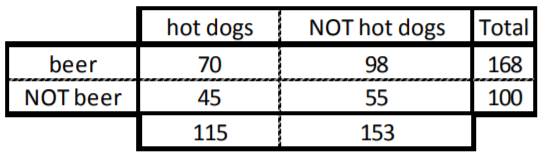
\includegraphics[height=0.2 \linewidth]{association/pict/beer_hotdog.png}
	\caption{es. birra - hot dog}
\end{figure}
Consideriamo le seguenti regole con le relative confidenze:
\begin{itemize}
	\item \{beer\} $\rightarrow$ \{hot dogs\} - confidence = $42\%$
	\item \{NOT beer\} $\rightarrow$ \{hot dogs\} - confidence = $45\%$
\end{itemize}	
Possiamo inferire che i clienti che acquistano birra sono meno inclini ($42\%$) ad acquistare hot dog rispetto a quelli che non acquistano birra ($45\%$).

Analizziamo ora gli stessi dati ma categorizzando se il cliente è single o no:
\begin{figure}[H]
	\centering
	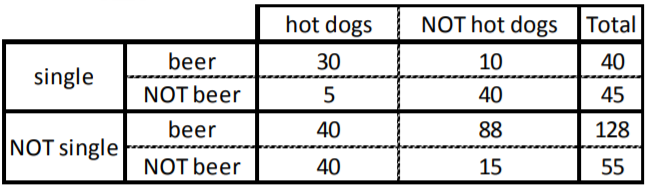
\includegraphics[height=0.2 \linewidth]{association/pict/beer_hotdog_single.png}
	\caption{es. cliente single: birra - hot dog}
\end{figure}
Pertanto posso derivare queste due coppie di regole:
\begin{itemize}
	\item Single
	\begin{itemize}
		\item \{beer\} $\rightarrow$ \{hot dogs\} - confidence = $75\%$
		\item \{NOT beer\} $\rightarrow$ \{hot dogs\} - confidence = $11\%$
	\end{itemize}
	\item NOT Single
	\begin{itemize}
		\item \{beer\} $\rightarrow$ \{hot dogs\} - confidence = $31\%$
		\item \{NOT beer\} $\rightarrow$ \{hot dogs\} - confidence = $73\%$
	\end{itemize}
\end{itemize}
Da questi dati posso affermare che: i single che acqustano birra sono più inclini ($75\%$) ad acquistare anche hot dog rispetto a quelli che non acquistano birra ($11\%$).\\

Quindi sia l'azienda di consulenza che il direttore del mini-market avevano ragione soltanto che per comprenderlo bisognava categorizzare i clienti. 

\paragraph{Paradosso di Simpson} o Yule-Simpson effect, è un paradosso della probabilità e statistica, in cui una tendenza appare in diversi gruppi di dati ma sparisce o si inverte quando questi gruppi sono combinati. \\

Bisogna applicare una appropriata stratificazione dei dati per evitare la generazione di associazioni spurie risultati dal paradosso di Simpson. 

Es. per i dati del market-basket, la catena di supermercati dovrebbe stratificarli secondo la location del negozio, mentre i dati sanitari da vari pazienti dovrebbero essere stratificati secondo fattori quali l'età o il genere.






\end{document}